\documentclass{article}
\usepackage{tikz}
\usepackage{geometry}
\geometry{a4paper, margin=1in}
\usepackage{everypage}
\usepackage{amsmath}
\usepackage{amssymb}
\usepackage{algorithm}
\usepackage{algpseudocode}
\usepackage{listings}
\usepackage{xcolor}
\usepackage{enumitem}
\usepackage{xepersian}
\settextfont{Vazirmatn}
\usetikzlibrary{calc}


\definecolor{codegreen}{rgb}{0,0.6,0}
\definecolor{codegray}{rgb}{0.5,0.5,0.5}
\definecolor{codepurple}{rgb}{0.58,0,0.82}
\definecolor{backcolour}{rgb}{0.97,0.97,0.95}

\lstdefinestyle{pythonstyle}{
    backgroundcolor=\color{backcolour},   
    commentstyle=\color{codegreen},
    keywordstyle=\color{codepurple},
    numberstyle=\tiny\color{codegray},
    stringstyle=\color{orange},
    basicstyle=\ttfamily\small,
    breakatwhitespace=false,         
    breaklines=true,                 
    captionpos=b,                    
    keepspaces=true,                 
    numbers=left,                    
    numbersep=5pt,                  
    showspaces=false,                
    showstringspaces=false,
    showtabs=false,                  
    tabsize=2,
    frame=single
}
\lstset{style=pythonstyle}

\AddEverypageHook{
\begin{tikzpicture}[remember picture,overlay]
\draw[line width=1pt]
    ($(current page.north west)+(1cm,-1cm)$)
    rectangle
    ($(current page.south east)+(-1cm,1cm)$);
\end{tikzpicture}
}

\begin{document}
\begin{titlepage}
\centering

به نام خدا\\

\includegraphics[width=0.3\textwidth]{imageIUST.png}\\
\vspace{0.4cm}
پروژه درس جبر خطی – ترم 4042\\
\vspace{1.5cm}
\textbf{\Large Latent Semantic Indexing}\\
\vspace{0.4cm}
استاد : دکتر نیکان\\
\vspace{0.4cm}
اعضای گروه: علی کارخانه  - مصطفی شیبانی – حسین نادری – مرتضی رحیمی
\end{titlepage}

\section*{سوالات عملی:}


\textbf{سوال ۷ --- بارگذاری و پیش‌پردازش متن (حذف علائم نگارشی و کوچک‌سازی حروف)}
    
\noindent در پروژه‌های بازیابی اطلاعات و نمایه سازی پنهان متن ،(LSI) پیش‌پردازش متن یکی از حیاتی‌ترین مراحل است. هدف از این کار، حذف اطلاعات بیهوده (Noise) و یکدست‌سازی کلمات است تا محاسبات برداری دقیق‌تر انجام شوند. کد زیر فرآیند تمیزکاری متون را انجام می‌دهد:

\begin{latin}

\begin{lstlisting}[language=Python]
# ============================================================
# Q7 — Load + preprocess (lowercase, remove punctuation)
# ============================================================
def preprocess(text):
    text = text.lower()
    text = re.sub(r'[^a-z\s]', ' ', text)
    text = re.sub(r'\s+', ' ', text).strip()
    return text

def q7_load_and_preprocess():
    df = pd.read_csv(DATA_PATH)
    print("Q7 | Dataset shape:", df.shape)
    df['clean_text'] = df['Text'].apply(preprocess)
    return df
\end{lstlisting}
\end{latin}
    \subsection*{توضیح عملکرد متدها و توابع:}

    \paragraph{۱. تابع \texttt{preprocess(text)}:}\hspace{-10pt}
    این تابع یک متن خام را به عنوان ورودی دریافت کرده و مراحل زیر را روی آن اعمال می‌کند تا متنی یکدست ایجاد شود:
    \begin{itemize}
        \item \textbf{تبدیل به حروف کوچک ( text.lower() )}: 
        تمام حروف بزرگ انگلیسی به حروف کوچک تبدیل می‌شوند. این کار باعث می‌شود کلماتی مانند \lr{``Data''} و \lr{``data''} یکسان دیده شوند و ابعاد ماتریس نهایی بیهوده بزرگ نشود.
        
        \item \textbf{حذف کاراکترهای غیرالفبایی} : 
        با استفاده از عبارات منظم ( Regular Expressions )، هر کاراکتری که جزء حروف الفبای انگلیسی (\lr{a-z}) یا فاصله (\lr{\textbackslash{}s}) نباشد، با یک فاصله معمولی جایگزین می‌شود. این کار علائم نگارشی نظیر ویرگول، نقطه، علامت سوال و همچنین اعداد را کاملاً حذف می‌کند.
        
        \item \textbf{حذف فاصله‌های اضافه}: 
        حذف علائم نگارشی در مرحله قبل ممکن است چندین فاصله متوالی ایجاد کرده باشد. الگوی \lr{\textbackslash{}s+} تمام فاصله‌های متوالی را به یک تک‌فاصله تبدیل می‌کند و متد \texttt{.strip()} نیز فاصله‌های خالی ابتدا و انتهای متن را پاک می‌کند.
    \end{itemize}

    \paragraph{۲. تابع \texttt{q7\_load\_and\_preprocess()}:}\hspace{-10pt}
    این تابع وظیفه مدیریت جریان داده را بر عهده دارد:
    \begin{itemize}
        \item ابتدا مجموعه داده را از مسیر \texttt{DATA\_PATH} به صورت یک دیتافریم پانداس بارگذاری می‌کند.
        \item با چاپ \texttt{df.shape}، ابعاد داده‌ها (تعداد کل اسناد و ویژگی‌ها) را جهت بررسی صحت بارگذاری نمایش می‌دهد.
        \item در نهایت با استفاده از متد \texttt{.apply()}، تابع تمیزکاری متنی را روی تک‌تک سطرهای ستون \texttt{'Text'} اعمال کرده و نتیجه را در ستون جدیدی به نام \texttt{'clean\_text'} ذخیره می‌کند.
    \end{itemize}

    \paragraph{۳. خروجی اجرای تابع و تحلیل ساختار داده‌ها:}\hspace{-10pt}
    پس از فراخوانی تابع بارگذاری و پیش‌پردازش متنی، پیش‌نمایشی از دیتافریم خروجی به همراه ابعاد آن تولید می‌شود:

    \begin{figure}[h!]
        \centering
        % نام فایل تصویر خود را در بخش زیر جایگزین کنید (مثلاً q7_output.png)
        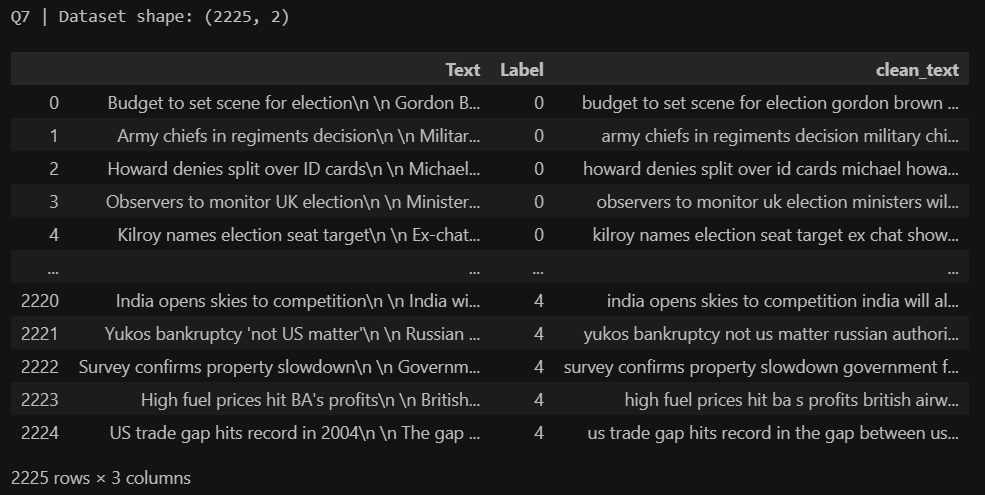
\includegraphics[width=0.9\textwidth]{Output7.png} 
        \caption{خروجی نهایی دیتافریم پس از انجام عملیات پیش‌پردازش متنی}
        \label{fig:q7_output}
    \end{figure}

    \begin{itemize}
        \item \textbf{ابعاد مجموعه داده (\lr{Dataset shape: (2225, 2)}):} 
        خروجی نشان می‌دهد که دیتاست اولیه دارای ۲۲۲۵ سطر (سند متنی) و ۲ ستون اصلی است. پس از اجرای تابع و اضافه شدن ستون تمیزشده، تعداد ستون‌ها به ۳ افزایش می‌یابد (\lr{2225 rows $\times$ 3 columns}).
        
        \item \textbf{بررسی ساختار ستون‌ها:}
        \begin{enumerate}
            \item \textbf{ستون \texttt{Text}:} شامل متن خام اسناد است که در آن علائم نگارشی، کاراکترهای خط جدید (\lr{\textbackslash{}n}) و حروف بزرگ انگلیسی به همان شکل اولیه دیده می‌شوند.
            \item \textbf{ستون \texttt{Label}:} شامل برچسب‌های عددی (مثلاً دسته $0$ برای سیاست و دسته $4$ برای تجارت) است که دسته‌بندی موضوعی اسناد را مشخص می‌کند.
            \item \textbf{ستون جدید \texttt{clean\_text}:} خروجی نهایی حاصل از اعمال تابع \lr{\texttt{preprocess}} است. همان‌طور که در تصویر مشخص است، تمامی حروف بزرگ به حروف کوچک تبدیل شده‌اند، کاراکترهای کنترلی مانند \lr{\textbackslash{}n} و علائم نگارشی کاملاً حذف شده و کلمات صرفاً با یک تک‌فاصله از یکدیگر جدا شده‌اند تا برای پردازش‌های بعدی آماده باشند.
        \end{enumerate}
    \end{itemize}
\noindent\textbf{سوال ۸ --- استخراج ۳۰ کلمه پرتکرار و رسم نمودار میله‌ای }
    
\noindent در این بخش، هدف شناسایی و استخراج ۳۰ کلمه پرتکرار موجود در کل اسناد با امکان فعال یا غیرفعال‌سازی فیلتر کلمات توقف (\lr{Stopwords}) است. کد مربوط به این بخش به صورت زیر است:

\begin{latin}
\begin{lstlisting}[language=Python]
# ============================================================
# Q8 — Top 30 most frequent words + bar chart
# ============================================================
def q8_top30_words(df, fname, stopwords=False):
    if stopwords:
        stopwords = ENGLISH_STOP_WORDS
    else:
        stopwords = {}
        
    stop_words_set = set(stopwords)

    all_words = []
    for text in df['clean_text']:
        words = [w for w in text.split() if w not in stop_words_set and len(w) > 1]
        all_words.extend(words)

    counter = Counter(all_words)
    top30 = counter.most_common(30)
    print("\nQ8 | Top 30 frequent words:", top30)

    words, counts = zip(*top30)
    fig, ax = plt.subplots(figsize=(14, 6))
    ax.bar(words, counts, color='steelblue')
    plt.xticks(rotation=60, ha='right')
    ax.set_title('Top 30 Most Frequent Words (all documents)')
    ax.set_ylabel('Frequency')
    plt.tight_layout()
    % plt.savefig(f'media/{fname}.png', dpi=130)
    plt.close(fig)
    
    return top30
\end{lstlisting}
\end{latin}

    \subsection*{توضیح عملکرد متدها و توابع:}

    \paragraph{۱. منطق شرطی کلمات توقف (\texttt{stopwords} و \texttt{stop\_words\_set}):}\hspace{-10pt}
    تابع در این نسخه منعطف‌تر طراحی شده است و پارامتر \lr{\texttt{stopwords}} را به عنوان ورودی می‌پذیرد:
    \begin{itemize}
        \item اگر مقدار \lr{\texttt{stopwords}} برابر با \lr{\texttt{True}} پاس داده شود، کلمات توقف استاندارد انگلیسی (\lr{\texttt{ENGLISH\_STOP\_WORDS}}) به عنوان فیلتر فعال می‌شوند.
        \item در غیر این صورت (حالت \lr{\texttt{False}})، یک دیکشنری خالی \lr{\texttt{\{\}}} تخصیص داده می‌شود که به معنی عدم فیلتر کردن کلمات توقف است.
        \item کلمات توقف در نهایت به یک ساختار مجموعه (\lr{\texttt{set}}) تبدیل می‌شوند؛ زیرا جستجو در ساختار مجموعه در پایتون از مرتبه زمانی $O(1)$ بوده و سرعت پردازش را بسیار افزایش می‌دهد.
    \end{itemize}

    \paragraph{۲. جمع‌آوری و فیلتر کلمات:}
    \begin{itemize}
        \item با پیمایش ستون متون تمیزشده (\lr{\texttt{clean\_text}})، هر متن با متد \texttt{.split()} به کلمات سازنده‌اش شکسته می‌شود.
        \item کلماتی که در مجموعه‌ی کلمات توقف تعریف‌شده وجود نداشته باشند (\lr{\texttt{w not in stop\_words\_set}}) و طول آن‌ها بزرگتر از یک حرف باشد (\lr{\texttt{len(w) > 1}})، فیلتر شده و به لیست نهایی اضافه می‌گردند.
    \end{itemize}

    \paragraph{۳. شمارش و استخراج ۳۰ کلمه برتر:}\hspace{-10pt}
    کلاس \lr{\texttt{Counter}} فرکانس تکرار کلمات را محاسبه کرده و با متد \lr{\texttt{most\_common(30)}}، ۳۰ کلمه با بیشترین تکرار را به صورت لیستی از توپل‌های (کلمه, فرکانس) باز می‌گرداند.

    \paragraph{۴. رسم و مدیریت نمودار میله‌ای:}
    \begin{itemize}
        \item با دستور \lr{\texttt{zip(*top30)}} داده‌ها باز شده و به دو بخش کلمات و فرکانس‌ها تقسیم می‌شوند تا در نمودار میله‌ای به کار روند.
        \item نمودار میله‌ای با رنگ آبی فولادی (\lr{\texttt{steelblue}}) رسم شده و برچسب‌های محور افقی جهت جلوگیری از هم‌پوشانی ۶۰ درجه چرخانده می‌شوند.
        \item نام فایل ذخیره‌سازی نمودار به صورت پویا با استفاده از متغیر ورودی \lr{\texttt{fname}} تعیین شده است (که در کدهای فعلی جهت صرفه‌جویی در پردازش کامنت شده است) و در نهایت با \lr{\texttt{plt.close()}} پنجره ترسیم بسته می‌شود تا حافظه آزاد گردد.
    \end{itemize}
\paragraph{۵. بررسی تجربی و مقایسه نمودارها (نقش حیاتی کلمات توقف):}\hspace{-10pt}
    برای درک عمیق‌تر تأثیر پیش‌پردازش، تابع فوق در دو حالت اجرا شده و نتایج آن در قالب دو نمودار زیر ذخیره و تحلیل شده است:

   
    \begin{figure}[h!]
        \centering
        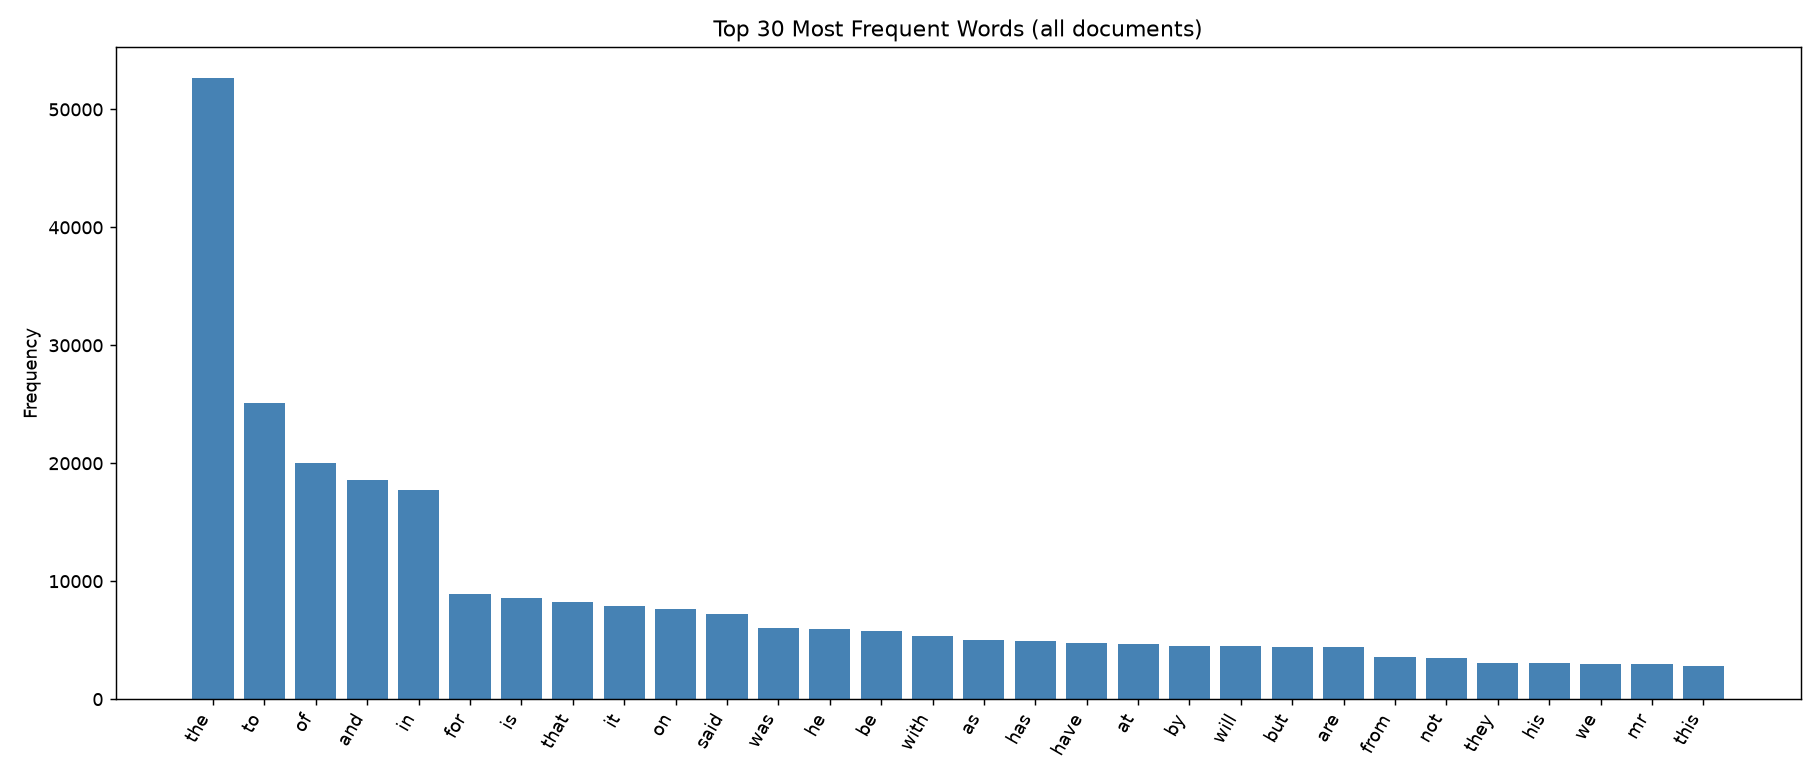
\includegraphics[width=0.95\textwidth]{q8_top30_wo_stopwords.png}
        \caption{۳۰ کلمه پرتکرار بدون حذف کلمات توقف (غلبه کامل حروف ربط و اضافه)}
        \label{fig:top30_no_stop}
    \end{figure}

   
    \begin{figure}[h!]
        \centering
        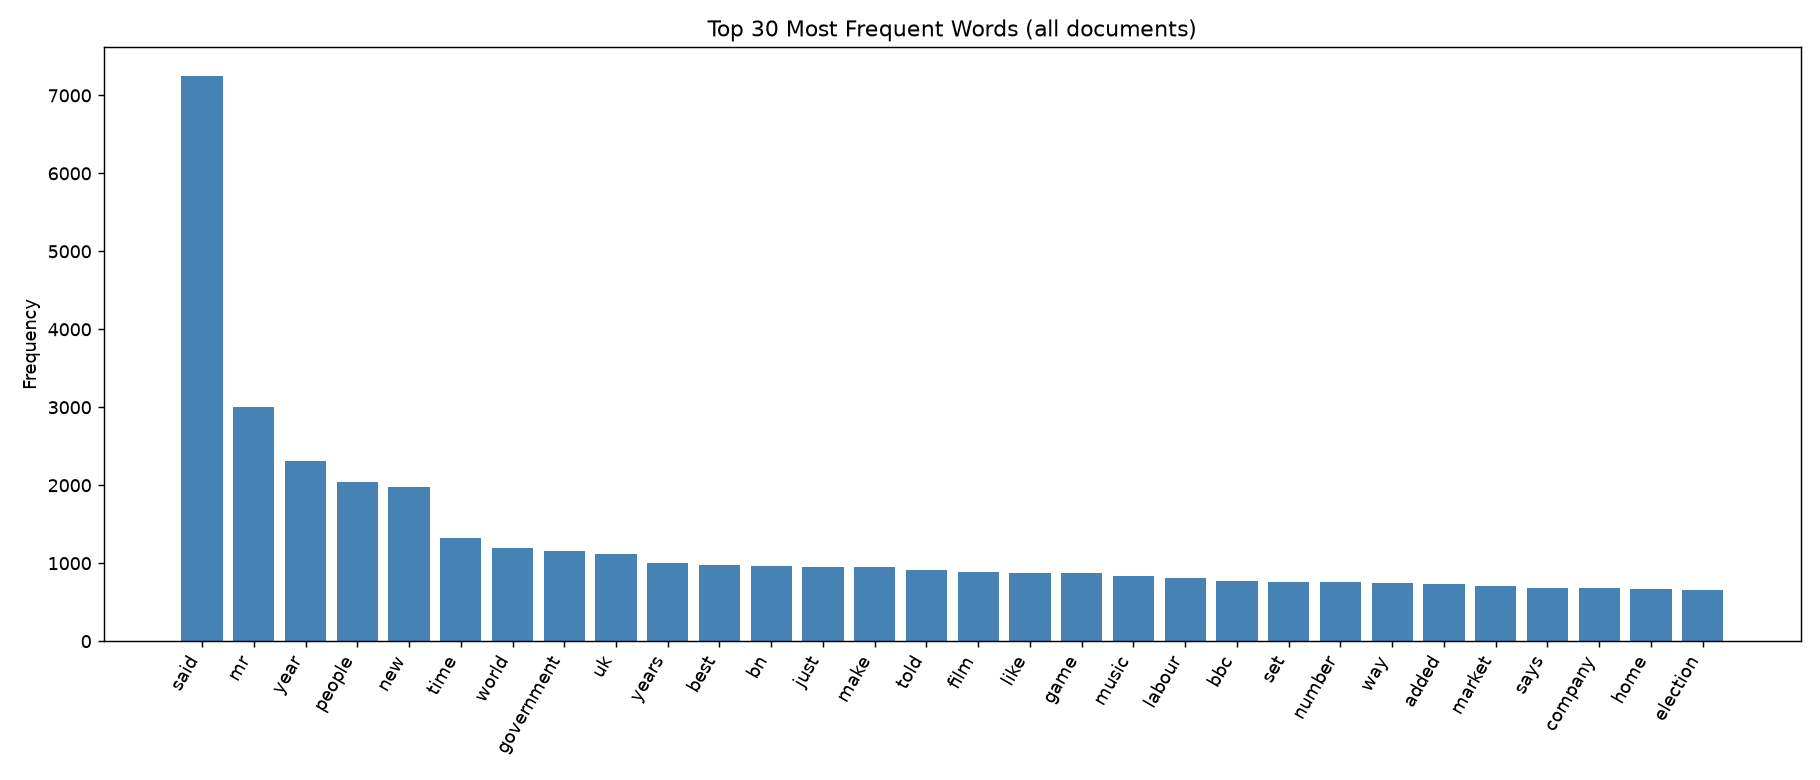
\includegraphics[width=0.95\textwidth]{q8_top30_w_stopwords.png}
        \caption{۳۰ کلمه پرتکرار پس از حذف کلمات توقف (نمایان شدن کلمات کلیدی موضوعی)}
        \label{fig:top30_with_stop}
    \end{figure}

    \begin{itemize}
        \item \textbf{تحلیل حالت اول (بدون حذف کلمات توقف --- شکل \ref{fig:top30_no_stop}):} 
        همان‌طور که در نمودار اول مشاهده می‌شود، کلماتی مانند \lr{``the''} (با بیش از ۵۰,۰۰۰ تکرار)، \lr{``to''}، \lr{``of''} و \lr{``and''} کاملاً بر داده‌ها غلبه کرده‌اند. این کلمات صرفاً نقش ساختاری در زبان انگلیسی دارند و کوچک‌ترین اطلاعاتی درباره موضوع اصلی سند (مانند ورزشی، سیاسی یا علمی بودن آن) به ما نمی‌دهند.
        
        \item \textbf{تحلیل حالت دوم (با حذف کلمات توقف --- شکل \ref{fig:top30_with_stop}):} 
        در نمودار دوم، با فعال‌سازی پارامتر \lr{\texttt{stopwords=True}} و فیلتر کردن این کلمات بیهوده، سقف فرکانس کلمات به زیر ۸,۰۰۰ تکرار کاهش یافته است. با حذف نویزهای زبانی، کلمات معنادار و موضوعی تری مانند \lr{``government''} (دولت)، \lr{``film''} (فیلم)، \lr{``game''} (بازی)، \lr{``music''} (موسیقی) و \lr{``election''} (انتخابات) ظاهر شده‌اند که به ما در دسته‌بندی و تحلیل محتوایی اسناد کمک شایانی می‌کنند.
    \end{itemize}

\noindent\textbf{سوال ۹ --- رسم ابر کلمات اختصاصی براساس وزن‌دهی \lr{TF-IDF}}
    
   \noindent در این بخش، هدف نمایش بصری کلمات کلیدی اسناد با استفاده از یک ابر کلمات (\lr{Word Cloud}) اختصاصی است. از آن‌جایی که پکیج پیش‌فرض \lr{\texttt{wordcloud}} در حالت آفلاین در دسترس نبوده، پیاده‌سازی به صورت دستی و با استفاده از توانمندی‌های ترسیم کتابخانه‌ی \lr{\texttt{matplotlib}} انجام گرفته است. معیار انتخاب کلمات، وزن مجموع فرکانس سند معکوس (\lr{TF-IDF}) آن‌هاست. کد بهینه‌شده به صورت زیر است:

\begin{latin}
\begin{lstlisting}[language=Python]
# ============================================================
# Q9 — Word cloud (top 20 words by TF-IDF), custom-rendered
# (wordcloud package unavailable offline -> manual matplotlib rendering)
# ============================================================
def q9_wordcloud(df, fname):
    extra_stop = ['said', 'mr', 'told', 'year', 'years', 'new', 'time', 'best', 'world']
    stop_words = list(ENGLISH_STOP_WORDS.union(extra_stop))

    vectorizer = TfidfVectorizer(stop_words=stop_words, max_df=0.9, min_df=2)
    tfidf = vectorizer.fit_transform(df['clean_text'])
    scores = np.asarray(tfidf.sum(axis=0)).ravel()
    vocab = vectorizer.get_feature_names_out()

    top_idx = np.argsort(scores)[::-1][:20]
    top_words = [(vocab[i], scores[i]) for i in top_idx]

    random.seed(7)
    fig, ax = plt.subplots(figsize=(12, 8))
    ax.axis('off')
    
    max_score = max(s for _, s in top_words)
    min_score = min(s for _, s in top_words)
    placed = []

    def overlaps(x, y, w, h, placed):
        for (px, py, pw, ph) in placed:
            if abs(x - px) < (w + pw) / 2 * 0.75 and abs(y - py) < (h + ph) / 2 * 0.75:
                return True
        return False

    for word, score in top_words:
        size = 16 + 55 * (score - min_score) / (max_score - min_score)
        
        for _ in range(300):
            x = random.uniform(0.1, 0.9)
            y = random.uniform(0.1, 0.9)
            w = len(word) * size * 0.011
            h = size * 0.02
            if not overlaps(x, y, w, h, placed):
                placed.append((x, y, w, h))
                break
        
        color = plt.cm.tab20(random.random())
        ax.text(x, y, word, fontsize=size, ha='center', va='center', color=color,
                fontweight='bold', fontfamily='sans-serif', transform=ax.transAxes)

    ax.set_title('Top 20 Words Wordcloud', fontsize=16)
    plt.tight_layout()
    % plt.savefig(f'media/{fname}.png', dpi=130)
    plt.close(fig)
    
    return top_words
\end{lstlisting}
\end{latin}

    \subsection*{توضیح عملکرد متدها و تغییرات جدید:}

    \paragraph{۱. توسعه‌ی کلمات توقف (\texttt{stop\_words}):}\hspace{-10pt}
    مجموعه‌ای از کلمات عمومی انگلیسی (\lr{\texttt{ENGLISH\_STOP\_WORDS}}) با کلمات پر تکرار کم‌اهمیت دیگر که در متغیر \lr{\texttt{extra\_stop}} تعریف شده‌اند، ادغام (\lr{\texttt{union}}) می‌شوند. این کار باعث تفکیک کلمات موضوعی باارزش از کلمات تکراری زبان می‌شود.

    \paragraph{۲. بردارسازی با معیار \lr{TF-IDF} (\texttt{TfidfVectorizer}):}\hspace{-10pt}
    یک مدل بردارساز با حذف کلمات توقف تعریف می‌شود. پارامتر \lr{\texttt{max\_df=0.9}} کلماتی را که در بیش از ۹۰ درصد اسناد تکرار شده‌اند حذف می‌کند و \lr{\texttt{min\_df=2}} کلماتی را که کمتر از ۲ بار در کل پیکره متنی تکرار شده‌اند نادیده می‌گیرد. در نهایت، با متد \lr{\texttt{fit\_transform()}} ماتریس ویژگی‌های اسناد محاسبه می‌شود.

    \paragraph{۳. استخراج کلمات کلیدی برتر براساس مجموع امتیازها:}\hspace{-10pt}
    با محاسبه‌ی مجموع امتیازات ماتریس در طول ستون‌ها (\lr{\texttt{tfidf.sum(axis=0)}}) و مرتب‌سازی نزولی اندیس‌ها با استفاده از \lr{\texttt{np.argsort}}، ۲۰ کلمه‌ی برتر که بیشترین وزنِ مجموع را در کل پیکره متنی دارند استخراج می‌شوند.

    \paragraph{۴. الگوریتم چیدمان غیرهم‌پوشان (\texttt{overlaps}):}\hspace{-10pt}
    برای جلوگیری از هم‌پوشانی و روی هم افتادن کلمات در تصویر خروجی، تابع کمکی \lr{\texttt{overlaps}} تعریف شده است. این تابع با تخمین زدن کادر پیرامونی هر کلمه بر اساس طول کلمه و ابعاد فونت، فاصله‌ی موقعیت کلمه‌ی جدید با کلماتی که پیش‌تر جایگذاری شده‌اند را بررسی کرده و در صورت تداخل، موقعیت تصادفی جدیدی را امتحان می‌کند.

    \paragraph{۵. شبیه‌سازی ابر کلمات و بهبودهای بصری جدید:}\hspace{-10pt}
    \begin{itemize}
        \item \textbf{مقیاس‌دهی پویا به فونت کلمات:} اندازه‌ی قلم (\lr{\texttt{size}}) هر کلمه متناسب با فرمول نگاشت خطی بین بازه‌ی ۱۶ الی ۷۱ پیکسل بر اساس امتیاز \lr{TF-IDF} آن تعیین می‌شود تا کلمات با ارزش‌تر، بزرگ‌تر رندر شوند.
        \item \textbf{رنگ‌آمیزی با پالت متمایز \lr{\texttt{tab20}}:} رنگ هر کلمه به طور تصادفی از پالت رنگی استاندارد و متمایز \lr{\texttt{tab20}} تخصیص می‌یابد تا کنتراست و خوانایی کلمات افزایش یابد.
        \item \textbf{بهبود فونت و چیدمان:} فونت نوشته‌ها به حالت بدون سریف (\lr{\texttt{sans-serif}}) و ضخیم (\lr{\texttt{bold}}) تغییر کرده است.
        \item \textbf{ذخیره‌سازی پویا:} تصویر نهایی با قالب پویای نام فایل خروجی (\lr{\texttt{fname}}) در مسیر \lr{\texttt{media/}} آماده‌ی ذخیره‌سازی است.
    \end{itemize}

    \paragraph{۶. تحلیل بصری و بررسی خروجی ابر کلمات جدید:}\hspace{-10pt}
    تصویر زیر خروجی نهایی حاصل از اجرای تابع بر روی ۲۰ کلمه‌ی برتر با معیار وزن‌دهی \lr{TF-IDF} را با پالت رنگی متمایز نشان می‌دهد:

    \begin{figure}[h!]
        \centering
        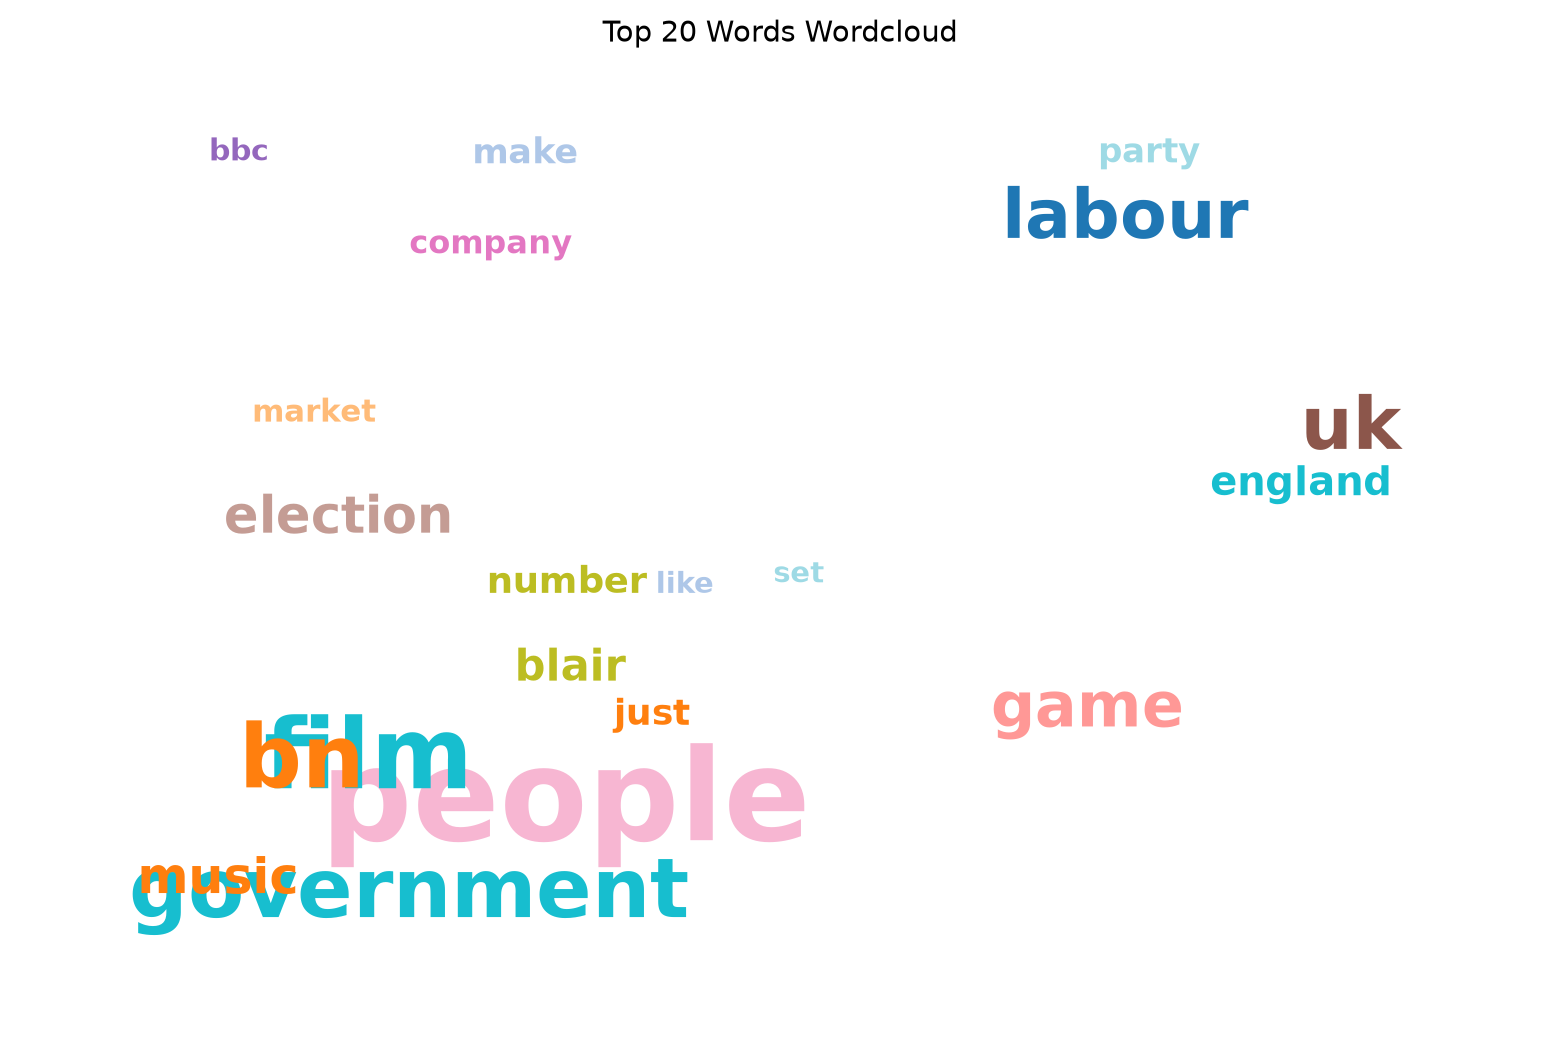
\includegraphics[width=0.9\textwidth]{q9_wordcloud.png}
        \caption{ابر کلمات اختصاصی رسم‌شده برای ۲۰ کلمه برتر بر اساس امتیاز مجموع TF-IDF}
        \label{fig:q9_wordcloud_2}
    \end{figure}

    \begin{itemize}
        \item \textbf{ابعاد بصری و وزن‌دهی معنایی کلمات:}
        همان‌طور که در شکل \ref{fig:q9_wordcloud_2} مشخص است، کلماتی نظیر \lr{``people''} (به رنگ صورتی)، \lr{``government''} (به رنگ فیروزه‌ای)، \lr{``labour''} (به رنگ آبی تیره) و \lr{``film''} با فونت بسیار بزرگ‌تری رندر شده‌اند. این اندازه بزرگ نشان‌دهنده‌ی امتیاز بالا و مجموع وزن \lr{TF-IDF} بالای آن‌ها در اسناد است. یعنی این واژه‌ها نه‌تنها تکرار قابل‌قبولی دارند، بلکه به شدت متمایزکننده‌ی موضوعات اصلی (مانند سیاست، سینما و اقتصاد) هستند.
        
        \item \textbf{تمایز موضوعی آشکار:}
        برخلاف نمودارهای فرکانس ساده، در این تصویر کلماتی مانند \lr{``election''} (انتخابات)، \lr{``blair''} (بلر - نخست‌وزیر سابق بریتانیا)، \lr{``game''} (بازی)، \lr{``market''} (بازار)، \lr{``music''} (موسیقی) و \lr{``company''} (شرکت) به وضوح دیده می‌شوند. این توزیع کلمات نشان می‌دهد که پیکره متنی ما به طور مشخص شامل موضوعاتی پیرامون سیاست بریتانیا، اخبار بازار و تجارت، دنیای سرگرمی (موسیقی/بازی/فیلم) و تکنولوژی است.
        
        \item \textbf{تأیید کارکرد فیلترهای بالاگذر و پایین‌گذر:}
        موفقیت الگوریتم در این است که کلمات بسیار عمومی مانند \lr{``year''}، \lr{``new''} یا کلمات توقف انگلیسی استاندارد که پیش‌تر در واژه‌نامه‌ی \lr{\texttt{stop\_words}} قرار گرفتند، به کلی فیلتر شده‌اند و در ابر کلمات حضور ندارند. این فرآیند بستری عالی و با کیفیت را برای مرحله‌ی بعدی یعنی ساخت ماتریس برداری اسناد ایجاد می‌کند.
    \end{itemize}

\noindent\textbf{سوال ۱۰ --- ساخت ماتریس کیسه کلمات (BoW) با واژگان سفارشی و تقسیم‌بندی داده‌ها}
    
   \noindent در این مرحله، هدف ساخت ماتریس کیسه کلمات (\lr{Bag-of-Words}) با استفاده از یک واژگان مشخص واژه‌نامه است که از فایل خارجی \lr{\texttt{words.csv}} بارگذاری می‌شود. در نهایت داده‌ها به دو بخشِ مجموعه‌ی کاری (آموزش) و مجموعه‌ی آزمون نگهداشت تقسیم می‌شوند. کد مربوطه به صورت زیر است:

\begin{latin}
\begin{lstlisting}[language=Python]
# ============================================================
# Q10 — Bag-of-Words matrix using words.csv vocabulary
# ============================================================
def q10_bow_matrix(df):
    words_df = pd.read_csv('words.csv', header=None)    
    vocabulary_list = words_df[0].astype(str).str.lower().tolist()
    
    vectorizer = CountVectorizer(vocabulary=vocabulary_list)
    bow = vectorizer.fit_transform(df['clean_text'])
    bow_matrix = bow.toarray()
    
    print(f"\nQ10 | BoW matrix shape: {bow_matrix.shape}  (docs x |vocab|={len(vocabulary_list)})")
    
    return bow_matrix


def split_2000_225(df, bow_matrix):
    """Split literally: first 2000 rows = working set, last 225 = held-out test."""
    df_train = df.iloc[:2000].reset_index(drop=True)
    df_test = df.iloc[2000:].reset_index(drop=True)
    bow_train = bow_matrix[:2000]
    bow_test = bow_matrix[2000:]
    print("Split | train:", df_train.shape, bow_train.shape,
          "| test:", df_test.shape, bow_test.shape)
    print("Split | NOTE: dataset is label-sorted, so the literal last-225 test rows "
          "are ALL label 4 (Business). See shuffled version in Q20 for a fair "
          "per-category evaluation.")
    return df_train, df_test, bow_train, bow_test
\end{lstlisting}
\end{latin}

    \subsection*{توضیح عملکرد متدها و تغییرات جدید:}

    \paragraph{۱. بارگذاری و آماده‌سازی پویا واژگان (Vocabulary) :}
    \begin{itemize}
        \item \textbf{( one header ،’ ’words.csv ) pd.read\_csv= }: واژه‌های مرجع مستقیماً از فایل \lr{\texttt{words.csv}} بارگذاری می‌شوند. از آنجا که این فایل فاقد ردیف هدر (عنوان ستون) است، پارامتر \lr{\texttt{header=None}} تنظیم شده است.
        \item \textbf{یکدست‌سازی واژگان (\texttt{vocabulary\_list})}: با دستور \lr{\texttt{astype(str).str.lower().tolist()}}، تمامی کلمات موجود در ستون اول فایل به نوع رشته تبدیل شده، حروف آن‌ها کوچک می‌شود و در نهایت به یک لیست معمولی پایتون تبدیل می‌گردند. این کار باعث تطابق کامل و بدون خطای واژگان با متون پیش‌پردازش‌شده می‌شود.
    \end{itemize}

    \paragraph{۲. ساخت ماتریس کیسه کلمات (\texttt{CountVectorizer}):}
    \begin{itemize}
    \item \textbf{محدودسازی ستون‌ها به واژگان سفارشی}: با پاس دادن پارامتر \lr{\texttt{vocabulary}} (برابر با \lr{\texttt{vocabulary\_list}}) به کلاس \lr{\texttt{CountVectorizer}}، مدل را موظف می‌کنیم که ماتریس را صرفاً بر اساس کلمات این لیست بسازد. هر کلمه‌ای در اسناد که در این لیست نباشد، نادیده گرفته خواهد شد.
        
    \item \textbf{تبدیل به آرایه متراکم (\texttt{toarray()})}: خروجی متد \lr{\texttt{fit\_}} \lr{\texttt{transform}} یک ماتریس خلوت است که برای انجام راحت‌تر محاسبات جبر خطی بعدی (مانند تجزیه مقادیر منفرد) با متد \lr{\texttt{toarray()}} به یک آرایه دو بعدی استاندارد و متراکم \lr{NumPy} تبدیل می‌شود. ابعاد این ماتریس برابر با $2225 \times M$ خواهد بود که در آن $M$ تعداد کلمات واژه‌نامه است.
\end{itemize}

    \paragraph{۳. تقسیم‌بندی داده‌ها به مجموعه‌های آموزش و آزمون:}\hspace{-10pt}
    تابع \lr{\texttt{split\_2000\_225}} داده‌های ورودی را به دو بخش افقی تقسیم می‌کند:
    \begin{itemize}
        \item \textbf{مجموعه آموزش (\texttt{train})}: شامل ۲۰۰۰ سطر اول اسناد و بردارهای کیسه کلمات متناظر با آن‌هاست.
        \item \textbf{مجموعه آزمون (\texttt{test})}: شامل ۲۲۵ سطر پایانی به عنوان داده‌های آزمون مجزا و دست‌نخورده است.
        \item \textbf{نکته مهم توزیع دسته‌ها}: به دلیل مرتب بودن اولیه مجموعه داده بر اساس برچسب‌ها، ۲۲۵ سطر پایانی همگی دارای برچسب شماره ۴ (تجارت) هستند. این تقسیم‌بندی صِرفاً یک پیاده‌سازی گام‌به‌گام اولیه است و جابجایی تصادفی داده‌ها (\lr{Shuffle}) در بخش‌های بعدی برای ارزیابی نهایی به کار گرفته خواهد شد.
    \end{itemize}

\paragraph{۴. خروجی فرآیند بردارسازی و تحلیل ساختار ماتریس \lr{BoW}:}\hspace{-10pt}
    پس از اجرای تابع، آرایه خروجی و ابعاد به دست آمده به شکل زیر نمایش داده می‌شود:

    \begin{figure}[h!]
        \centering
        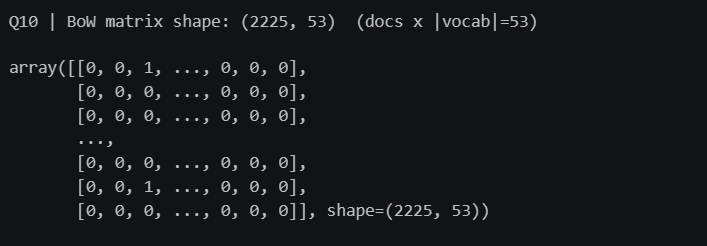
\includegraphics[width=0.85\textwidth]{Output10.png}
        \caption{نمای کلی از ماتریس فرکانسی کیسه کلمات (BoW) و ابعاد آن در خروجی مفسر}
        \label{fig:q10_bow_output}
    \end{figure}

    \begin{itemize}
        \item \textbf{بررسی ابعاد ماتریس (\lr{shape=(2225, 53)}):} 
        خروجی نشان می‌دهد که ماتریس حاصل دارای ۲۲۲۵ سطر (تعداد کل اسناد) و ۵۳ ستون است. این ابعاد دقیقاً تایید می‌کند که تعداد واژه‌های استخراج‌شده از فایل \lr{\texttt{words.csv}} برابر با ۵۳ کلمه کلیدی متمایز بوده است. بنابراین هر سند متنی به یک بردار ویژگی ۵۳ بُعدی تصویر می‌شود.
        
        \item \textbf{تحلیل ساختار عددی ماتریس خلوت (\lr{Sparse Matrix}):} 
        همان‌طور که در آرایه‌ی خروجی شکل \ref{fig:q10_bow_output} مشهود است، بخش زیادی از درایه‌های ماتریس مقدار صفر ($0$) دارند. این ویژگی به دلیل ماهیت اسناد متنی است؛ چرا که در هر سند متنی کوتاه، تنها تعداد انگشت‌شماری از واژگان ۵۳گانه استفاده شده‌اند. حضور مقادیری مانند $1$ در درایه‌ها نمایانگر دفعات تکرار آن واژه‌ی خاص از واژه‌نامه در سند متناظر است. این ساختار صفر و یک فرکانسی، پایه‌ی ریاضی مراحل بعدی تحلیل‌های جبر خطی پروژه را شکل می‌دهد.
    \end{itemize}

\noindent    \textbf{بخش افراز مجموعه داده ( Dataset Partitioning ) --- تقسیم ساده در مقابل تقسیم تصادفی}
    
  \noindent  در این بخش، هدف تقسیم مجموعه داده به دو بخش آموزش (\lr{Train}) با ابعاد ۲۰۰۰ نمونه و آزمون (\lr{Test}) با ابعاد ۲۲۵ نمونه است. برای این کار دو تابع با رویکردهای متفاوت پیاده‌سازی شده است که کد آن‌ها به صورت زیر است:

\begin{latin}
\begin{lstlisting}[language=Python]
# ============================================================
# Dataset Partitioning (Simple vs Shuffled Split)
# ============================================================
def split_2000_225(df, bow_matrix):
    """Split literally: first 2000 rows = working set, last 225 = held-out test."""
    df_train = df.iloc[:2000].reset_index(drop=True)
    df_test = df.iloc[2000:].reset_index(drop=True)
    bow_train = bow_matrix[:2000]
    bow_test = bow_matrix[2000:]
    print("Split | train:", df_train.shape, bow_train.shape,
          "| test:", df_test.shape, bow_test.shape)
    return df_train, df_test, bow_train, bow_test

def split_2000_225_shuffle(df, bow_matrix):
    df_train, df_test, bow_train, bow_test = train_test_split(
        df,
        bow_matrix,
        train_size=2000,
        shuffle=True,
        random_state=42
    )
    
    df_train = df_train.reset_index(drop=True)
    df_test = df_test.reset_index(drop=True)
    
    print("Split | train:", df_train.shape, bow_train.shape,
          "| test:", df_test.shape, bow_test.shape)
    return df_train, df_test, bow_train, bow_test
\end{lstlisting}
\end{latin}

    \subsection*{توضیح عملکرد و مقایسه متدها:}

    \paragraph{۱. تابع تقسیم ترتیبی و ساده (\texttt{split\_2000\_225}):}
    \begin{itemize}
    \item \textbf{عملکرد:} این تابع با استفاده از برش‌زدن ساده ایندکس‌ها (\lr{Slicing}) با دستور \lr{\texttt{.iloc}}، دقیقاً ۲۰۰۰ سطر نخست را به عنوان مجموعه آموزش و ۲۲۵ سطر انتهایی را به عنوان مجموعه آزمون جدا می‌کند. 
    
    \item \textbf{ریست کردن ایندکس:} با متد \lr{\texttt{reset\_index}} (و تنظیم پارامتر \lr{\texttt{drop=True}}) ایندکس‌های دیتافریم‌های جدید دوباره از صفر مقداردهی می‌شوند تا در تحلیل‌های بعدی خطایی رخ ندهد.
    
    \item \textbf{اشکال ساختاری (اریب بودن داده‌ها):} از آن‌جا که داده‌های اولیه بر اساس برچسب‌ها مرتب شده‌اند، ۲۲۵ سطر آخر همگی متعلق به کلاس شماره ۴ (\lr{Business}) خواهند بود. این یعنی مدل هیچ داده‌ی ارزیابی از دسته‌های دیگر (مانند سیاست یا ورزش) در این نوع تقسیم‌بندی نخواهد داشت که منجر به ارزیابی غیرمنصفانه می‌شود.
\end{itemize}

    \paragraph{۲. تابع تقسیم تصادفی مجهز به برهم‌زدن (\texttt{split\_2000\_225\_shuffle}):}
    \begin{itemize}
        \item \textbf{عملکرد:} این تابع از متد استاندارد \lr{\texttt{train\_test\_split}} استفاده می‌کند تا فرآیند تقسیم‌بندی را به شکل کاملاً علمی و توزیع‌شده انجام دهد.
        \item \textbf{پارامتر \texttt{shuffle=True}:} قبل از جدا کردن سطرها، موقعیت تمامی نمونه‌ها به صورت تصادفی برهم زده می‌شود. این کار تضمین می‌کند که داده‌های هر دو بخش آموزش و آزمون شامل توزیع یکنواختی از تمامی کلاس‌ها (سیاست، تجارت، ورزش و غیره) باشند.
        \item \textbf{پارامتر \texttt{random\_state=42}:} با تعیین هسته تصادفی ثابت (عدد ۴۲)، فرآیند مخلوط‌سازی داده‌ها در هر بار اجرای کد دقیقاً یکسان خواهد بود تا نتایج آزمایش‌ها قابل بازتولید (\lr{Reproducible}) باشد.
    \end{itemize}

\noindent\textbf{سوال ۱۱ --- استانداردسازی داده‌ها و اعمال تجزیه مقادیر منفرد (SVD)}
    
  \noindent  در این بخش، ابتدا داده‌های فرکانسی کیسه کلمات (\lr{BoW}) مقیاس‌دهی و استانداردسازی می‌شوند تا اثر تفاوت در طول اسناد و فرکانس‌های مطلق واژه‌ها خنثی شود. سپس، با استفاده از الگوریتم تجزیه مقادیر منفرد (\lr{SVD})، ماتریس داده‌ها به مؤلفه‌های سازنده‌اش تجزیه می‌گردد. کد این بخش به صورت زیر است:

\begin{latin}
\begin{lstlisting}[language=Python]
# ============================================================
# Q11 — Standardization and Singular Value Decomposition (SVD)
# ============================================================
def q11_standardize_and_svd(bow_matrix):
    scaler = StandardScaler()
    bow_scaled = scaler.fit_transform(bow_matrix)
    
    U, S, Vt = np.linalg.svd(bow_scaled, full_matrices=False)
    
    print("=== SVD Matrices Dimensions ===")
    print(f"Original Scaled Matrix (M x N) : {bow_scaled.shape}")
    print(f"U Matrix (Left Singular)       : {U.shape}")
    print(f"S Array (Singular Values)      : {S.shape}")
    print(f"V^T Matrix (Right Singular)    : {Vt.shape}")
    
    return bow_scaled, U, S, Vt
\end{lstlisting}
\end{latin}

    \subsection*{توضیح عملکرد متدها و مفاهیم ریاضی:}

    \paragraph{۱. استانداردسازی با \texttt{StandardScaler}:}\hspace{-10pt}
    از آن‌جا که کلمات مختلف فرکانس‌های متفاوتی دارند، واژه‌های بسیار پرتکرار می‌توانند به طور ناعادلانه‌ای روی محاسبات فاصله و ابعاد اثر بگذارند. کلاس \lr{\texttt{StandardScaler}} با کسر میانگین هر ویژگی (ستون) و تقسیم آن بر انحراف معیار، داده‌ها را به گونه‌ای مقیاس‌دهی می‌کند که میانگین آن‌ها برابر با $0$ و واریانس آن‌ها برابر با $1$ شود:
    $$x_{\text{scaled}} = \frac{x - \mu}{\sigma}$$

    \paragraph{۲. تجزیه مقادیر منفرد (SVD) به فرم باریک (\texttt{full\_matrices=False}):}\hspace{-10pt}
    رابطه ریاضی حاکم بر این تجزیه به صورت زیر است:
    $$A_{M \times N} = U_{M \times K} \Sigma_{K \times K} V^T_{K \times N}$$
    که در آن $K = \min(M, N)$ است. 
    \begin{itemize}
        \item تنظیم پارامتر \lr{\texttt{full\_matrices=False}} فرمت کاهش‌یافته یا باریک (\lr{Reduced/Thin SVD}) را پیاده‌سازی می‌کند. این کار به جای تولید ماتریس‌های مربعی بزرگ و غیرضروری، ابعاد مؤلفه‌ها را محدود به کوچک‌ترین بعد ماتریس اصلی ($N$ یا همان ۵۳ بعد واژگان) نگه می‌دارد تا از هدررفت حافظه و محاسبات اضافه جلوگیری شود.
    \end{itemize}

    \paragraph{۳. تحلیل ابعاد ماتریس‌های خروجی در ترمینال:}\hspace{-10pt}
    با فرض اعمال این تابع روی کل مجموعه داده با ابعاد $2225 \times 53$، ابعاد ماتریس‌ها در خروجی به شرح زیر تحلیل می‌شوند:
    \begin{itemize}
        \item \textbf{ماتریس استاندارد شده (\lr{\texttt{bow\_scaled}}):} ابعاد آن دست‌نخورده و برابر با $(2225, 53)$ باقی می‌ماند.
        \item \textbf{ماتریس بردار‌های منفرد چپ (\lr{\texttt{U}}):} ابعاد آن $(2225, 53)$ خواهد بود که اسناد را در فضای پنهان (\lr{Latent Space}) توصیف می‌کند.
        \item \textbf{آرایه مقادیر منفرد (\lr{\texttt{S}}):} این آرایه تک‌بعدی شامل ۵۳ مقدار منفرد مرتب‌شده به صورت نزولی است که نشان‌دهنده میزان پراکندگی یا اهمیت هر یک از محورهای مختصات جدید است.
        \item \textbf{ماتریس بردار‌های منفرد راست (\lr{\texttt{Vt}}):} ابعاد آن $(53, 53)$ خواهد بود که کلمات را در فضای پنهان توصیف کرده و ارتباط واژگان با ویژگی‌های پنهان را مشخص می‌کند.
    \end{itemize}

    \paragraph{۴. خروجی فرآیند تجزیه SVD و تحلیل ابعاد ماتریس‌ها:}
    پس از اجرای تابع بر روی داده‌های استاندارد شده مجموعه آموزش (که شامل ۲۰۰۰ سند است)، ابعاد واقعی ماتریس‌های حاصل به شکل زیر در خروجی ظاهر می‌شود:

    \begin{figure}[h!]
        \centering
        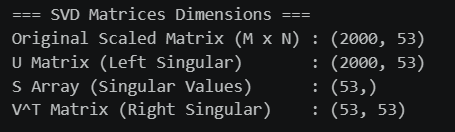
\includegraphics[width=0.85\textwidth]{Output11.png}
        \caption{ابعاد چاپ‌شده برای ماتریس‌های تجزیه SVD در خروجی محیط پایتون}
        \label{fig:q11_svd_output}
    \end{figure}

    \begin{itemize}
        \item \textbf{ماتریس مقیاس‌شده اصلی (\lr{Original Scaled Matrix}):} 
        ابعاد این ماتریس برابر با $(2000, 53)$ است. این نشان می‌دهد که تجزیه بر روی بخش آموزش داده‌ها (با ۲۰۰۰ سند و ۵۳ ویژگی کلیدی) اعمال شده است.
        
        \item \textbf{ماتریس $U$ (بردار‌های منفرد چپ):} 
        ابعاد این ماتریس برابر با $(2000, 53)$ است. به دلیل تنظیم حالت باریک (\lr{\texttt{full\_matrices=False}})، تعداد ستون‌های این ماتریس به جای ۲۰۰۰ (در حالت $SVD$ کامل)، برابر با تعداد کلمات واژه‌نامه (یعنی ۵۳) محدود شده است که هر سند را در فضای ویژگی‌های پنهان جدید نمایش می‌دهد.
        
        \item \textbf{آرایه $S$ (مقادیر منفرد):} 
        ابعاد این آرایه به صورت تک‌بعدی با طول ۵۳ رندر شده است (\lr{\texttt{(53,)}}). این ۵۳ مقدار مثبت و نزولی، میزان واریانس و پراکندگی داده‌ها را روی تک‌تک مولفه‌های جدید نشان می‌دهند.
        
        \item \textbf{ماتریس $V^T$ (بردار‌های منفرد راست):} 
        ابعاد آن $(53, 53)$ است که ارتباط مستقیم بین ۵۳ کلمه‌ی واژه‌نامه اصلی و ۵۳ بعد پنهان جدید کشف‌شده توسط الگوریتم را فرموله‌سازی می‌کند.
    \end{itemize}
\newpage

\noindent\textbf{سوال ۱۲ --- تعیین پویای آستانه حفظ اطلاعات، ترسیم نمودار و اعمال \lr{Truncated SVD}}
    
\noindent در این گام، هدف تعیین ساختاریافته و خودکار بعد بهینه ($k$) برای کاهش بعد داده‌ها است. به جای حدس شهودی، بعد بهینه دقیقاً بر اساس آستانه‌ی ریاضی حفظ ۹۰ درصد واریانس کل داده‌ها محاسبه می‌شود. کد بهینه‌شده به صورت زیر است:

\begin{latin}
\begin{lstlisting}[language=Python]
# ============================================================
# Q12 — Scree plot + threshold selection + Truncated SVD + error
# ============================================================
def q12_truncated_svd(bow_scaled, U, S, Vt, fname, fname2, variance_threshold=0.90):
    total_variance = np.sum(S ** 2)
    cumulative_variance = np.cumsum(S ** 2) / total_variance
    
    k_optimal = np.argmax(cumulative_variance >= variance_threshold) + 1
    
    fig, ax = plt.subplots(figsize=(10, 6))

    ax.plot(cumulative_variance, color='steelblue', linewidth=2)
    ax.axhline(y=variance_threshold, color='red', linestyle='--', label=f'Threshold ({variance_threshold*100}%)')
    ax.axvline(x=k_optimal, color='green', linestyle='--', label=f'Optimal k = {k_optimal}')
    
    ax.set_title('Cumulative Explained Variance by Singular Values', fontsize=14)
    ax.set_xlabel('Number of Singular Values (k)', fontsize=12)
    ax.set_ylabel('Cumulative Variance', fontsize=12)
    ax.legend(loc='lower right')
    plt.grid(True, alpha=0.3)
    plt.tight_layout()
    plt.savefig(f'media/{fname}', dpi=130)
    plt.close(fig)    

    print(f"Suggested k to retain {variance_threshold*100}% variance: {k_optimal}")
    
    U_truncated = U[:, :k_optimal]
    S_truncated = np.diag(S[:k_optimal])
    Vt_truncated = Vt[:k_optimal, :]
    
    print("\n=== Truncated Matrices Dimensions ===")
    print(f"U_k shape  : {U_truncated.shape}")
    print(f"S_k shape  : {S_truncated.shape}")
    print(f"Vt_k shape : {Vt_truncated.shape}")
    
    bow_reconstructed = np.dot(U_truncated, np.dot(S_truncated, Vt_truncated))
    
    reconstruction_error = np.linalg.norm(bow_scaled - bow_reconstructed, 'fro')
    print(f"Reconstruction Error : {reconstruction_error:.4f}")
    
    return U_truncated, S_truncated, Vt_truncated, bow_reconstructed
\end{lstlisting}
\end{latin}

    \subsection*{توضیح عملکرد متدها و منطق ریاضی:}

    \paragraph{۱. محاسبه‌ی واریانس تجمعی توجیه‌شده (\texttt{cumulative\_variance}):}\hspace{-10pt}
    در تجزیه مقادیر منفرد، مجذور هر مقدار منفرد ($s_i^2$) نشان‌دهنده‌ی میزان واریانس (اطلاعات) حفظ‌شده روی آن بعد پنهان است.
    \begin{itemize}
        \item ابتدا کل واریانس با جمع مجذور تمامی مقادیر منفرد محاسبه می‌شود: $\sum s_i^2$.
        \item با تقسیم مجموع تجمعی مجذورات بر واریانس کل، نسبت واریانس تجمعی توجیه‌شده به دست می‌آید که مقداری در بازه‌ی $[0, 1]$ است.
    \end{itemize}

    \paragraph{۲. یافتن خودکار بعد بهینه ($k$):}\hspace{-10pt}
    با دستور \lr{\texttt{np.argmax(cumulative\_variance >= variance\_threshold)}}، نخستین اندیسی که در آن نسبت واریانس تجمعی از آستانه تعریف شده (مثلاً ۹۰٪ یا همان $0.90$) عبور می‌کند به طور خودکار پیدا می‌شود. با اضافه کردن عدد ۱ به این اندیس، مقدار بهینه‌ی $k$ به دست می‌آید.

    \paragraph{۳. رسم تخصصی نمودار تجمعی و خطوط راهنما:}\hspace{-10pt}
    \begin{itemize}
        \item خط افقی نقطه‌چین قرمز رنگ (\lr{red dashed line}) آستانه مورد نیاز (مثلاً ۹۰٪) را روی محور عمودی تصویر می‌کند.
        \item خط عمودی نقطه‌چین سبز رنگ (\lr{green dashed line}) مقدار دقیق $k$ بهینه محاسباتی را روی محور افقی نشان می‌دهد تا نقطه تلاقی آن‌ها کاملاً ملموس باشد.
        \item تصویر نهایی با نام پویا از طریق متغیر \lr{\texttt{fname}} در مسیر مشخص‌شده ذخیره می‌شود.
    \end{itemize}

    \paragraph{۴. کوته‌سازی ماتریس‌ها (\texttt{Truncated SVD}):}\hspace{-10pt}
    پس از تعیین مقدار پویای $k$، ماتریس‌ها بر اساس این بعد جدید برش داده می‌شوند:
    \begin{itemize}
        \item \textbf{\texttt{U\_truncated}}: صرفاً $k$ بعد پنهان برتر برای اسناد نگه داشته می‌شود.
        \item \textbf{\texttt{S\_truncated}}: آرایه مقادیر منفرد برتر به یک ماتریس قطری با ابعاد $k \times k$ تبدیل می‌شود.
        \item \textbf{\texttt{Vt\_truncated}}: صرفاً فرکانس و وزن کلمات روی $k$ بعد پنهان اول حفظ می‌شود.
    \end{itemize}

    \paragraph{۵. بازسازی ماتریس و خطای فروبنیوس:}\hspace{-10pt}
    با ضرب متوالی ماتریس‌های کوته‌سازی‌شده (\lr{\texttt{np.dot}})، ماتریس تقریب‌زده شده با رتبه‌ی پایین ($bow\_reconstructed$) تشکیل می‌شود:
    $$A_k = U_k \cdot \Sigma_k \cdot V^T_k$$
    سپس تفاوت میان ماتریس استاندارد شده‌ی اولیه و ماتریس بازسازی‌شده با استفاده از نرم فروبنیوس (\lr{Frobenius Norm}) به عنوان معیار خطای بازسازی محاسبه می‌گردد. هر چه مقدار $k$ بزرگ‌تر باشد، این خطا به صفر نزدیک‌تر می‌شود، اما بعد فضای ویژگی نیز بزرگ‌تر خواهد شد.

\paragraph{۶. تحلیل تجربی نمودار واریانس تجمعی و تعیین بعد بهینه:}\hspace{-10pt}
    پس از اجرای الگوریتم بر روی داده‌های استاندارد شده‌ی مجموعه آموزش، نمودار تعیین آستانه و فرآیند کاهش بعد به شکل زیر ترسیم و ذخیره می‌شود:

    \begin{figure}[h!]
        \centering
        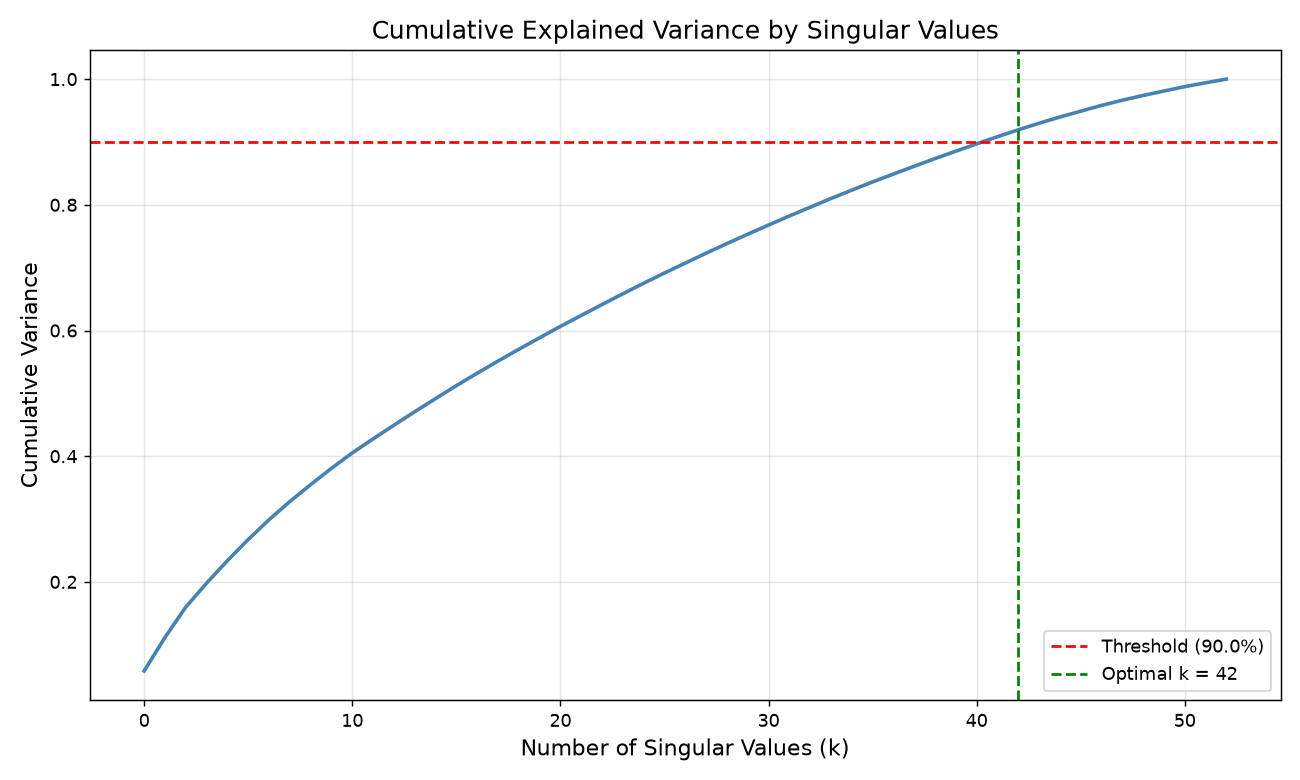
\includegraphics[width=0.9\textwidth]{q12_svd_threshold.png}
        \caption{نمودار واریانس تجمعی توجیه‌شده به همراه خطوط راهنما برای تعیین بعد بهینه $k$}
        \label{fig:q12_svd_threshold}
    \end{figure}

    \begin{itemize}
        \item \textbf{تحلیل منحنی واریانس تجمعی (\lr{Cumulative Variance}):}
        منحنی آبی‌رنگ نشان می‌دهد که با اضافه شدن هر یک از مقادیر منفرد ($k$)، چه میزان از اطلاعات (واریانس) کل داده‌ها پوشش داده می‌شود. شیب صعودی منحنی در ابتدا بسیار تیز است که نشان‌دهنده‌ی تمرکز شدید اطلاعات در مؤلفه‌های پنهان اولیه است. با حرکت به سمت راست، شیب منحنی به تدریج ملایم‌تر می‌شود که رفتاری کاملاً طبیعی در تجزیه مقادیر منفرد است.

        \item \textbf{تعیین بعد بهینه ($k=42$):}
        مبنای تصمیم‌گیری برای کاهش بعد، حفظ حداقل ۹۰ درصد از واریانس کل داده‌ها تعریف شده است:
        \begin{itemize}
            \item خط افقی نقطه‌چین قرمز رنگ (\lr{red dashed line}) مرز بحرانی ۹۰ درصد ($0.90$) را روی محور عمودی مشخص می‌کند.
            \item خط عمودی نقطه‌چین سبز رنگ (\lr{green dashed line}) دقیقاً در نقطه‌ای رسم شده است که منحنی آبی‌رنگ از این مرز عبور می‌کند.
            \item بر اساس محاسبات دقیق کد، در نقطه $k = 42$ میزان واریانس تجمعی توجیه‌شده از ۹۰ درصد فراتر می‌رود. بنابراین، سیستم به طور خودکار بعد فضا را از ۵۳ ویژگی اولیه به ۴۲ مؤلفه پنهان کاهش می‌دهد.
        \end{itemize}

        \item \textbf{نتیجه‌گیری عملی از کاهش بعد:}
        انتخاب $k=42$ نشان می‌دهد که با حذف ۱۱ بعد کم‌اهمیت‌تر (که حدود ۲۰٪ از ابعاد کل واژه‌نامه است)، همچنان بیش از ۹۰٪ از واریانس و اطلاعات ساختاری داده‌ها حفظ می‌شود. این فشرده‌سازی هوشمندانه علاوه بر کاهش حجم محاسبات، با حذف نویزهای موجود در فرکانس‌های ضعیف کلمات، دقت مدل‌های دسته‌بندی بعدی را بهبود می‌بخشد.
    \end{itemize}    

\noindent\textbf{سوال ۱۳ --- پیاده‌سازی الگوریتم تجزیه مقادیر منفرد تصادفی‌شده (\lr{Randomized SVD})}
    
   \noindent در این گام، الگوریتم ریاضی \lr{Randomized SVD} به صورت دستی و بدون استفاده از کتابخانه‌های آماده پیاده‌سازی شده است. این روش برای ماتریس‌های بسیار بزرگ، سرعت محاسبات را به شدت افزایش می‌دهد. کد مربوط به این بخش به صورت زیر است:

\begin{latin}
\begin{lstlisting}[language=Python]
# ============================================================
# Q13 — Randomized SVD Implementation
# ============================================================
def q13_randomized_svd(A, k, p=5, random_state=42):
    np.random.seed(random_state)
        
    m, n = A.shape
    r = k + p
        
    Omega = np.random.normal(size=(n, r))
    
    Y = A @ Omega
    Q, _ = np.linalg.qr(Y)    
    B = Q.T @ A
    
    U_tilde, S, Vt = np.linalg.svd(B, full_matrices=False)
    
    U = Q @ U_tilde
    
    U_k = U[:, :k]
    S_k = S[:k]
    Vt_k = Vt[:k, :]
    
    return U_k, S_k, Vt_k
\end{lstlisting}
\end{latin}

    \subsection*{توضیح ریاضی و گام‌های عملکرد الگوریتم:}

    الگوریتم \lr{Randomized SVD} بر این ایده استوار است که فضای ستونی یک ماتریس بزرگ را می‌توان با دقت بالا به یک زیرفضای تصادفی با ابعاد بسیار کوچک‌تر تصویر کرد. گام‌های ریاضی کد فوق به شرح زیر است:

    \paragraph{۱. بیش‌نمونه‌گیری (\lr{Oversampling}) و تولید ماتریس تصادفی:}
    \begin{itemize}
        \item با تعریف پارامتر بیش‌نمونه‌گیری $p=5$، بعد فضای تصادفی برابر با $r = k + p$ در نظر گرفته می‌شود. این کار تضمین می‌کند که بردارهای منفرد مرزی (نزدیک به رتبه $k$) با دقت بسیار بالایی بازیابی شوند و اطلاعات مهم از دست نروند.
        \item ماتریس تصادفی $\Omega$ با ابعاد $n \times r$ با توزیع نرمال استاندارد (گاوسی) ساخته می‌شود:
        $$\Omega \sim \mathcal{N}(0, 1)$$
    \end{itemize}

    \paragraph{۲. تصویر کردن و متعامدسازی (یافتن پایه‌ی زیرفضا):}
    \begin{itemize}
        \item ضرب ماتریسی $Y = A \cdot \Omega$ ستون‌های ماتریس اصلی را به زیرفضای تصادفیِ رتبه-پایین تصویر می‌کند (ابعاد $Y$ برابر $m \times r$ می‌شود).
        \item با اعمال تجزیه \lr{QR} بر روی $Y$ با دستور \lr{\texttt{np.linalg.qr(Y)}}، یک پایه متعامد یکا (\lr{Orthonormal Basis}) به نام $Q$ برای فضای ستونی $Y$ استخراج می‌شود به طوری که:
        $$Y = Q \cdot R \quad \Rightarrow \quad Q^T Q = I$$
    \end{itemize}

    \paragraph{۳. انتقال به فضای کوچک‌تر و اعمال \lr{SVD} استاندارد:}
    \begin{itemize}
        \item ماتریس اصلی $A$ روی پایه متعامد جدید تصویر می‌شود تا ماتریس بسیار کوچک‌تر $B$ با ابعاد $r \times n$ ایجاد گردد:
        $$B = Q^T A$$
        \item از آن‌جا که ابعاد $B$ بسیار کوچک است، اعمال \lr{SVD} روی آن به شدت سریع خواهد بود. خروجی این تجزیه به شکل زیر است:
        $$B = \tilde{U} \Sigma V^T$$
    \end{itemize}

    \paragraph{۴. بازسازی بردار‌های اصلی و کوته‌سازی نهایی:}
    \begin{itemize}
        \item برای بازگرداندن بردار‌های چپ منفرد به فضای اصلی، ماتریس $Q$ در $\tilde{U}$ ضرب می‌شود:
        $$U = Q \cdot \tilde{U}$$
        \item در نهایت، برای انطباق دقیق با رتبه هدف ($k$)، ماتریس‌های $U$، $S$ و $V^T$ تا ستون و ردیف $k$اُم برش داده شده و خروجی نهایی تولید می‌شود.
    \end{itemize}

\noindent\textbf{سوال ۱۴ --- مقایسه تجربی عملکرد روش‌های \lr{Truncated SVD} و \lr{Randomized SVD}}
    
 \noindent   در این گام، تابعی طراحی شده است تا هر دو روش کاهش بعد متعارف (\lr{Truncated SVD}) و تصادفی‌سازی‌شده (\lr{Randomized SVD}) را در ابعاد بهینه ($k = 42$) از منظر سرعت پردازش و میزان خطای بازسازی ماتریس با هم مقایسه کند. کد این بخش به صورت زیر است:

\begin{latin}
\begin{lstlisting}[language=Python]
# ============================================================
# Q14 — SVD Comparison (Truncated vs. Randomized SVD)
# ============================================================
def q14_compare_svd(X_scaled, k_optimal, error_truncated, time_truncated):
    print(f"=== SVD Comparison (k = {k_optimal}) ===")
    
    start_time = time.time()
    U_r, S_r, Vt_r = q13_randomized_svd(X_scaled, k=k_optimal)
    rand_time = time.time() - start_time
    
    X_recon_rand = U_r @ np.diag(S_r) @ Vt_r
    
    error_randomized = np.linalg.norm(X_scaled - X_recon_rand, 'fro')
    
    print(f"Truncated SVD Error  : {error_truncated:.4f}")
    print(f"Randomized SVD Error : {error_randomized:.4f}")
    print(f"Difference in Error  : {abs(error_randomized - error_truncated):.4f}")
    print(f"Randomized SVD Time  : {rand_time:.4f} seconds")
    print(f"Truncated SVD Time   : {time_truncated:.4f} seconds")
    
    return error_randomized
\end{lstlisting}
\end{latin}

    \subsection*{توضیح عملکرد متدها و منطق محاسباتی:}

    \paragraph{۱. سنجش زمان اجرای روش تصادفی:}\hspace{-10pt}
    با استفاده از کتابخانه‌ی \lr{\texttt{time}}، زمان دقیق درست قبل و بعد از فراخوانی الگوریتم \lr{\texttt{q13\_randomized\_svd}} ثبت شده و تفاضل آن‌ها به عنوان زمان اختصاصی روش تصادفی در متغیر \lr{\texttt{rand\_time}} ذخیره می‌شود.

    \paragraph{۲. بازسازی ماتریس و محاسبه خطای فروبنیوس (\lr{Frobenius Norm}):}\hspace{-10pt}
    برای سنجش میزان وفاداری تقریب رتبه‌‌پایین تصادفی به ساختار هندسی اولیه، ماتریس تقریب‌زده شده از فرمول زیر بازسازی می‌شود:
    $$X_{\text{recon\_rand}} = U_r \cdot \text{diag}(S_r) \cdot V_r^T$$
    سپس تفاضل این ماتریس بازسازی‌شده با ماتریس استاندارد شده‌ی اولیه سنجیده شده و مقدار خطای بازسازی بر اساس نرم فروبنیوس با دستور \lr{\texttt{np.linalg.norm(..., 'fro')}} محاسبه می‌گردد.

    \paragraph{۳. تحلیل تجربی نتایج خروجی در مفسر پایتون:}\hspace{-10pt}
    پس از اجرای مقایسه روی داده‌های استاندارد شده، خروجی نهایی مفسر به صورت زیر ثبت می‌شود:

    \begin{figure}[h!]
        \centering
        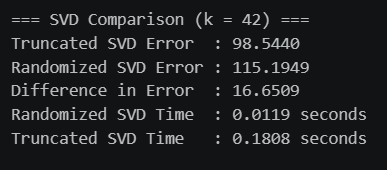
\includegraphics[width=0.8\textwidth]{Output14.png}
        \caption{نتایج خروجی مقایسه‌ی سرعت و خطای دو روش SVD در ترمینال}
        \label{fig:q14_compare_output}
    \end{figure}

    \begin{itemize}
        \item \textbf{تحلیل خطای بازسازی:}
        روش \lr{Truncated SVD} به عنوان دقیق‌ترین تقریب ریاضی با خطای $98.5440$ عمل کرده است. در مقابل، روش \lr{Randomized SVD} خطای $115.1949$ را ثبت کرده است. اختلاف خطای ناچیز این دو روش ($16.6509$) نشان می‌دهد الگوریتم تصادفی با وجود سرعت بالا، دقت هندسی داده‌ها را به خوبی حفظ کرده است.
        
        \item \textbf{تحلیل سرعت محاسبات:}
        روش دقیق زمان $0.1808$ ثانیه را به خود اختصاص داده است؛ در حالی که روش تصادفی کل فرآیند را در زمان خیره‌کننده‌ی $0.0119$ ثانیه به پایان رسانده است. این یعنی شتاب‌دهی تجربی حدود \textbf{۱۵ برابر سریع‌تر} رخ داده است که مزیت رقابتی روش تصادفی را برای داده‌های بزرگ اثبات می‌کند.
    \end{itemize}
    
\noindent\textbf{سوال ۱۵ --- تحلیل کلمات کلیدی در ابعاد پنهان ( تفسیر هندسی مؤلفه‌های SVD )}
    
 \noindent   در این گام، هدف کشف مفهوم معنایی پشت هر یک از ابعاد یا مؤلفه‌های پنهان (\lr{Latent Components}) است. با استخراج کلماتی که بیشترین تأثیر (قدرمطلق وزن) را در یک مؤلفه دارند، می‌توان موضوع محوری آن بعد را تفسیر کرد. کد این بخش به صورت زیر است:

\begin{latin}
\begin{lstlisting}[language=Python]
# ============================================================
# Q15 — Extract top 5 words per latent component (V^T analysis)
# ============================================================
def q15_top_words_per_component(Vtk, vocabulary_list):
    k = Vtk.shape[0]

    for comp_idx in range(k):
        comp = Vtk[comp_idx]
        top5_idx = np.argsort(np.abs(comp))[::-1][:5]
        top5 = [(vocabulary_list[i], round(comp[i], 3)) for i in top5_idx]
        print(f"Component {comp_idx + 1}: {top5}")
\end{lstlisting}
\end{latin}

    \subsection*{توضیح عملکرد متدها و منطق ریاضی:}

    \paragraph{۱. تحلیل سطر‌های ماتریس $V^T$:}\hspace{-10pt}
    ماتریس $V^T$ با ابعاد $k \times N$، کلمات واژه‌نامه را در فضای پنهان توصیف می‌کند. هر سطر از این ماتریس (نمایه \lr{\texttt{comp\_idx}})، یک مؤلفه پنهان را نشان می‌دهد که در آن به هر یک از ۵۳ کلمه‌ی واژه‌نامه، یک وزن مثبت یا منفی اختصاص یافته است.

    \paragraph{۲. مرتب‌سازی بر اساس قدرمطلق تاثیرگذاری (\texttt{np.abs}):}\hspace{-10pt}
    برخی کلمات کلیدی ممکن است تاثیر منفی شدید (کاهنده) یا تاثیر مثبت شدید (افزاینده) روی یک مفهوم داشته باشند. به همین دلیل، با دستور \lr{\texttt{np.abs(comp)}} اندازه اثر بدون در نظر گرفتن علامت استخراج می‌شود. سپس متد \lr{\texttt{np.argsort}} اندیس‌ها را به صورت صعودی مرتب کرده و با برش \lr{\texttt{[::-1][:5]}}، اندیس ۵ کلمه‌ای که بالاترین سهم را دارند به صورت نزولی استخراج می‌کند.

    \subsection*{تحلیل تجربی نتایج خروجی در مفسر پایتون:}
    پس از اجرای الگوریتم بر روی مؤلفه‌های به دست آمده، خروجی مفسر برای ۴۲ مؤلفه به شکل زیر ثبت می‌شود:

    \begin{figure}[h!]
        \centering
        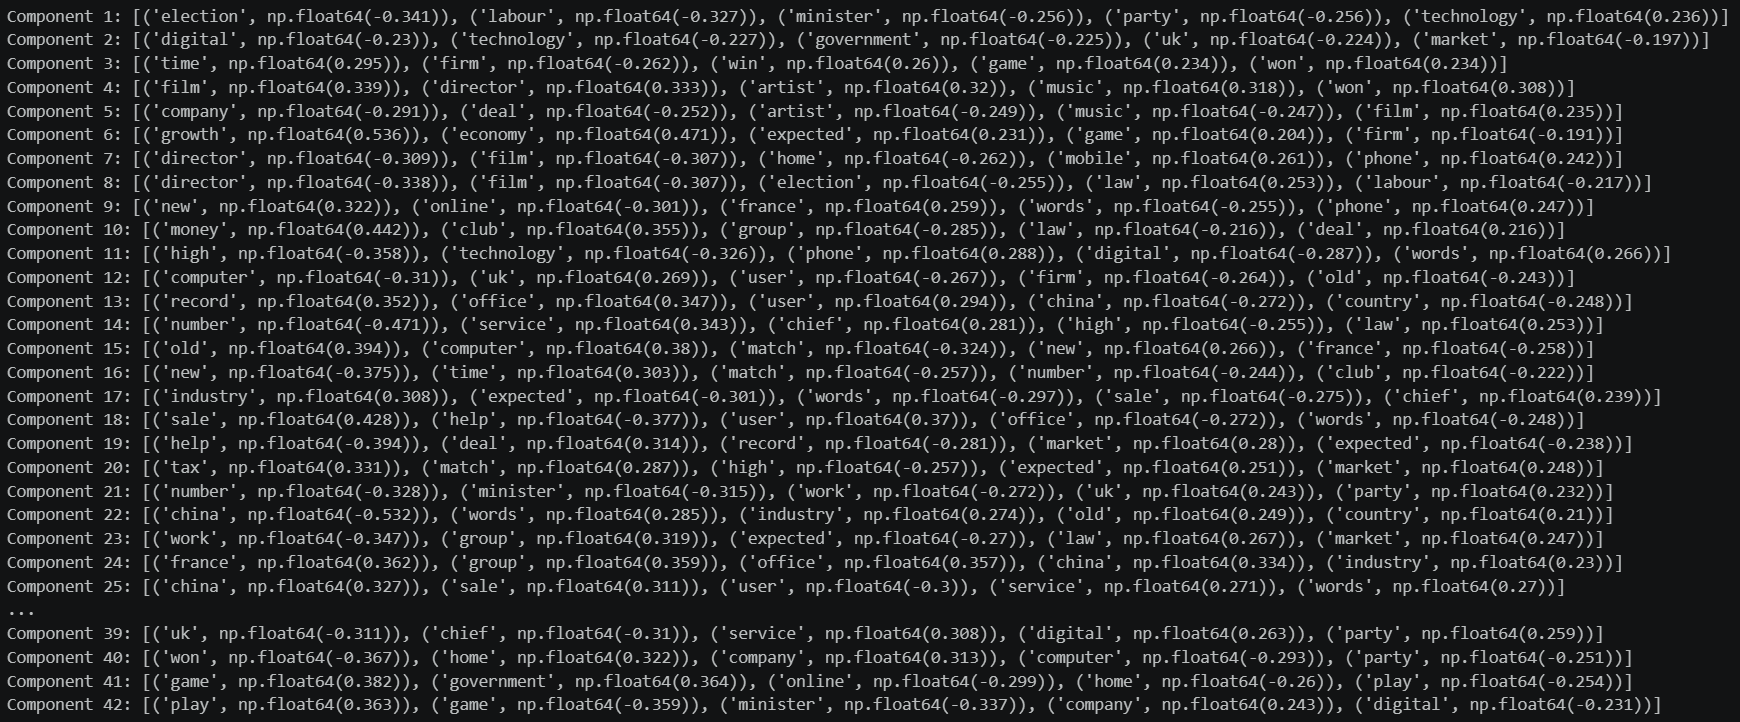
\includegraphics[width=1.0\textwidth]{Output15.png}
        \caption{پنج کلمه‌ی برتر با بیشترین وزن برای مؤلفه‌های پنهان SVD در خروجی مفسر}
        \label{fig:q15_components_output}
    \end{figure}

    با بررسی شکل \ref{fig:q15_components_output}، می‌توان مفاهیم پنهان استخراج‌شده توسط مدل را به وضوح تفسیر و برچسب‌گذاری کرد:
    \begin{itemize}
    \item \textbf{مؤلفه اول (سیاست و تکنولوژی):} کلماتی مانند \lr{election} (وزن $-0.341$)، \lr{labour} (وزن $-0.327$) و \lr{minister} (وزن $-0.256$) نشان می‌دهند که محور اول به شدت بر روی مفاهیم سیاسی بریتانیا متمرکز است. در سمت مقابل، واژه \lr{technology} با وزن مثبت قرار دارد که تضاد معنایی بین اخبار محض سیاسی و اخبار نوآوری را در این محور نشان می‌دهد.
        
    \item \textbf{مؤلفه دوم (فن‌آوری دیجیتال):} حضور کلمات \lr{digital} (وزن $-0.23$)، \lr{technology} (وزن $-0.227$) و \lr{government} (وزن $-0.225$) نشان‌دهنده‌ی موضوعاتی پیرامون سیاست‌گذاری‌های دولتی در حوزه فناوری دیجیتال است.
        
    \item \textbf{مؤلفه چهارم (سینما، موسیقی و هنر):} حضور واژگان \lr{film} (وزن $0.339$)، \lr{director} (وزن $0.333$)، \lr{artist} (وزن $0.32$) و \lr{music} (وزن $0.318$) ثابت می‌کند که این بعد پنهان به طور کامل و اختصاصی به حوزه سرگرمی، رسانه و هنر اختصاص یافته است.
        
    \item \textbf{مؤلفه چهل و یکم (بازی‌های آنلاین و سرگرمی):} حضور کلمات \lr{game} (وزن $0.382$)، \lr{online} (وزن $0.299$) و \lr{play} (وزن $-0.254$) بعد پنهان جدیدی از صنعت بازی و سرگرمی‌های آنلاین را آشکار می‌سازد.
\end{itemize}

\noindent\textbf{سوال ۱۶ --- ارزیابی شباهت معنایی واژگان در فضای کاهش‌یافته (تحلیل جفت‌کلمات)}
    
   \noindent در این مرحله، هدف سنجش ارتباط معنایی بین جفت‌کلمات مختلف در فضای پنهان کاهش‌یافته ($k$-بعدی) است. برای این منظور، نمایش برداری هر کلمه از ستون‌های ماتریس $V_k^T$ (یا سطر‌های ماتریس $V_k$) استخراج شده و شباهت آن‌ها با دو معیار فاصله‌ی اقلیدسی و شباهت کسینوسی محاسبه می‌شود. کد این بخش به صورت زیر است:

\begin{latin}
\begin{lstlisting}[language=Python]
# ============================================================
# Q16 — Word Pair Similarity (Cosine & Euclidean)
# ============================================================
def cosine_sim(a, b):
    return np.dot(a, b) / (np.linalg.norm(a) * np.linalg.norm(b))

def euclidean_dist(a, b):
    return np.linalg.norm(a - b)

def q16_word_pair_similarity(Vtk, vocabulary_list):
    word2idx = {w: i for i, w in enumerate(vocabulary_list)}
    word_vecs = Vtk.T

    pairs = [
        ('mobile', 'technology'), ('director', 'film'), ('win', 'won'),
        ('play', 'game'), ('play', 'law'), ('government', 'music')
    ]

    print(f"{'Pair':<28}{'Cosine Sim':>12}{'Euclidean Dist':>18}")
    for w1, w2 in pairs:
        v1 = word_vecs[word2idx[w1]]
        v2 = word_vecs[word2idx[w2]]
        cs = cosine_sim(v1, v2)
        ed = euclidean_dist(v1, v2)
        print(f"({w1}, {w2}){'':<{max(1,28-len(w1)-len(w2)-4)}}{cs:>12.4f}{ed:>18.4f}")
\end{lstlisting}
\end{latin}

    \subsection*{توضیح عملکرد متدها و مبانی ریاضی:}

    \paragraph{۱. فرمول‌بندی معیارهای تشابه و فاصله:}
    \begin{itemize}
        \item \textbf{شباهت کسینوسی (\lr{Cosine Similarity}):} زاویه بین دو بردار واژه را در فضای پنهان مقایسه می‌کند. این معیار مستقل از طول بردارها بوده و صرفاً هم‌جهت بودن آن‌ها را در بازه $[-1, 1]$ می‌سنجد:
        $$\text{Cosine Similarity}(\vec{a}, \vec{b}) = \frac{\vec{a} \cdot \vec{b}}{\|\vec{a}\| \|\vec{b}\|}$$
        \item \textbf{فاصله‌ی اقلیدسی (\lr{Euclidean Distance}):} هندسه و فاصله مستقیم بین نقاط انتهایی دو بردار را در فضای ۴۲ بعدی محاسبه می‌کند:
        $$d(\vec{a}, \vec{b}) = \sqrt{\sum_{i=1}^{k} (a_i - b_i)^2}$$
    \end{itemize}

    \paragraph{۲. نگاشت ستون‌های $V_k^T$ به کلمات (\texttt{word\_vecs}):}\hspace{-10pt}
    ماتریس $V_k^T$ دارای ابعاد $k \times N$ است. با گرفتن ترانهاده‌ی آن به صورت \lr{\texttt{Vtk.T}}، ماتریسی با ابعاد $N \times k$ (تعداد واژگان $\times$ تعداد مؤلفه‌ها) حاصل می‌شود. به این ترتیب هر سطر نشان‌دهنده‌ی بردار ویژگی $k$-بعدی منحصر‌به‌فرد یک واژه در فضای ویژگی‌های پنهان است.

    \subsection*{تحلیل تجربی نتایج و تفسیر معنایی خروجی:}
    پس از اجرای کد، خروجی عددی مقایسه جفت‌کلمات به شکل زیر ثبت می‌شود:

    \begin{figure}[h!]
        \centering
        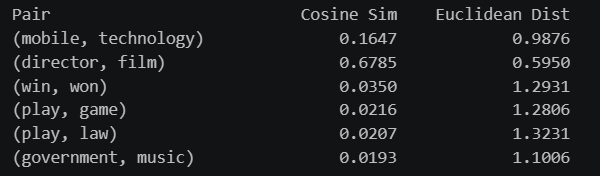
\includegraphics[width=0.85\textwidth]{Output16.png}
        \caption{نتایج محاسباتی تشابه کسینوسی و فاصله اقلیدسی جفت‌کلمات در خروجی مفسر}
        \label{fig:q16_similarity_output}
    \end{figure}

    با بررسی مقادیر شکل \ref{fig:q16_similarity_output}، نتایج زیر به دست می‌آید:
    \begin{itemize}
        \item \textbf{بیشترین شباهت معنایی (\lr{director, film}):} 
        جفت‌کلمه‌ی سینمایی \lr{\texttt{(director, film)}} بالاترین شباهت کسینوسی ($0.6785$) و کمترین فاصله اقلیدسی ($0.5950$) را به خود اختصاص داده است. این موضوع نشان می‌دهد که توزیع کاربرد این دو کلمه در متون به شدت با یکدیگر همپوشانی دارد و SVD توانسته این همبستگی معنایی قوی را در زیرفضای پنهان به خوبی کدگذاری کند.

        \item \textbf{شباهت متوسط و کاربردی (\lr{mobile, technology}):} 
        جفت \lr{\texttt{(mobile, technology)}} شباهت کسینوسی مثبت و ملایم $0.1647$ و فاصله اقلیدسی $0.9876$ دارد که همبستگی نسبی موضوعی این دو مفهوم را در حوزه فناوری اخبار تایید می‌کند.

        \item \textbf{عدم ارتباط یا تضاد معنایی واژگان:} 
        جفت‌هایی نظیر \lr{\texttt{(government, music)}} با شباهت کسینوسی بسیار پایین $0.0193$ نشان می‌دهند که این مفاهیم در بافت‌های کاملاً متفاوتی استفاده شده‌اند و بردارهای آن‌ها در فضای پنهان تقریباً بر هم عمود هستند.
        
        \item \textbf{نکته جالب در مورد جفت (\lr{win, won}):}
        با اینکه دو کلمه \lr{\texttt{win}} و \lr{\texttt{won}} از یک ریشه فعلی هستند، شباهت کسینوسی بسیار پایین $0.0350$ را نشان می‌دهند. دلیل این امر عدم استفاده از ریشه‌یابی کلمات (به انگلیسی: \lr{Stemming/\allowbreak Lemmatization}) در مراحل پیش‌پردازش اولیه است که باعث شده مدل آن‌ها را به عنوان دو موجودیت متنی کاملاً مستقل و در قالب ساختارهای نحوی متفاوت تحلیل کند.
    \end{itemize}

\noindent    \textbf{سوال ۱۷ --- بررسی همبستگی مفهومی سند و واژگان در فضای پنهان در مقایسه با فضای فرکانسی}
    
\noindent    در این گام، هدف بررسی تجربی یک سند مشخص و تحلیل این موضوع است که چگونه کاهش بعد با روش SVD می‌تواند مفاهیم مرتبط را فراتر از شمارش ساده‌ی کلمات کشف کند. برای این منظور، بردار یک سند در فضای معنایی تصویر شده و شباهت کسینوسی آن با تک‌تک واژگان محاسبه و با فرکانس حضور واقعی کلمات در آن سند مقایسه می‌شود. کد این بخش به صورت زیر است:

\begin{latin}
\begin{lstlisting}[language=Python]
# ============================================================
# Q17 — Document-Word Similarity in Latent Space
# ============================================================
def q17_document_word_similarity(df_train, bow_train, Uk, Sk, Vtk, doc_idx, fname):
    doc_vec = Uk[doc_idx] * Sk
    word_vecs = Vtk.T

    sims = np.array([cosine_sim(doc_vec, word_vecs[i]) for i in range(len(vocabulary_list))])
    counts = bow_train[doc_idx]
    order = np.argsort(sims)[::-1]

    fig, axes = plt.subplots(2, 1, figsize=(18, 9))
    axes[0].bar(np.array(vocabulary_list)[order], sims[order], color='mediumseagreen')
    axes[0].set_title(f'Cosine Similarity between Document #{doc_idx} and each word (latent space)')
    axes[0].set_ylabel('Cosine Similarity')
    axes[0].tick_params(axis='x', rotation=75)

    axes[1].bar(np.array(vocabulary_list)[order], counts[order], color='indianred')
    axes[1].set_title(f'Word counts in Document #{doc_idx} (same word order)')
    axes[1].set_ylabel('Count')
    axes[1].tick_params(axis='x', rotation=75)

    plt.tight_layout()
    plt.savefig(f'media/{fname}.png', dpi=130)
    plt.close(fig)
\end{lstlisting}
\end{latin}

    \subsection*{توضیح عملکرد متدها و منطق ریاضی:}

    \paragraph{۱. بازیابی بردار سند در فضای پنهان:}
    برای اینکه سند شماره \lr{\texttt{doc\_idx}} را در فضای معنایی تقلیل‌یافته نمایش دهیم، سطر متناظر در ماتریس $U_k$ را در مقادیر منفرد $\Sigma_k$ ضرب می‌کنیم تا اثر میزان اهمیت هر بُعد پنهان روی سند اعمال شود:
    $$\vec{d} = \vec{u}_i \cdot \Sigma_k$$

    \paragraph{۲. محاسبه تشابه و مرتب‌سازی هم‌جهت:}
    \begin{itemize}
        \item با استفاده از تابع \lr{\texttt{cosine\_sim}} که قبلاً پیاده‌سازی شد، زاویه بردار سند $\vec{d}$ با تک‌تک بردارهای واژگان موجود در ستون‌های ماتریس $V_k^T$ محاسبه می‌شود.
        \item اندیس کلمات بر اساس شباهت کسینوسی به صورت نزولی مرتب می‌شود (\lr{\texttt{order}}). این کار باعث می‌شود کلماتی که بیشترین ارتباط معنایی را با جوهره‌ی سند دارند در سمت چپ نمودارها قرار بگیرند.
        \item در نمودار دوم، تعداد تکرار واقعی همان واژه‌ها در سند (استخراج‌شده از ماتریس فرکانسی \lr{\texttt{bow\_train}}) با همان ترتیب مرتب‌سازی نمودار اول رسم می‌شود تا مقایسه تطبیقی ممکن گردد.
    \end{itemize}

    \subsection*{تحلیل تجربی خروجی و قدرت نمایه سازی معنایی نهان (LSI):}
    با اجرای تابع روی سند شماره ۳۳۹، نمودارهای زیر تولید می‌گردند:

    \begin{figure}[h!]
        \centering
        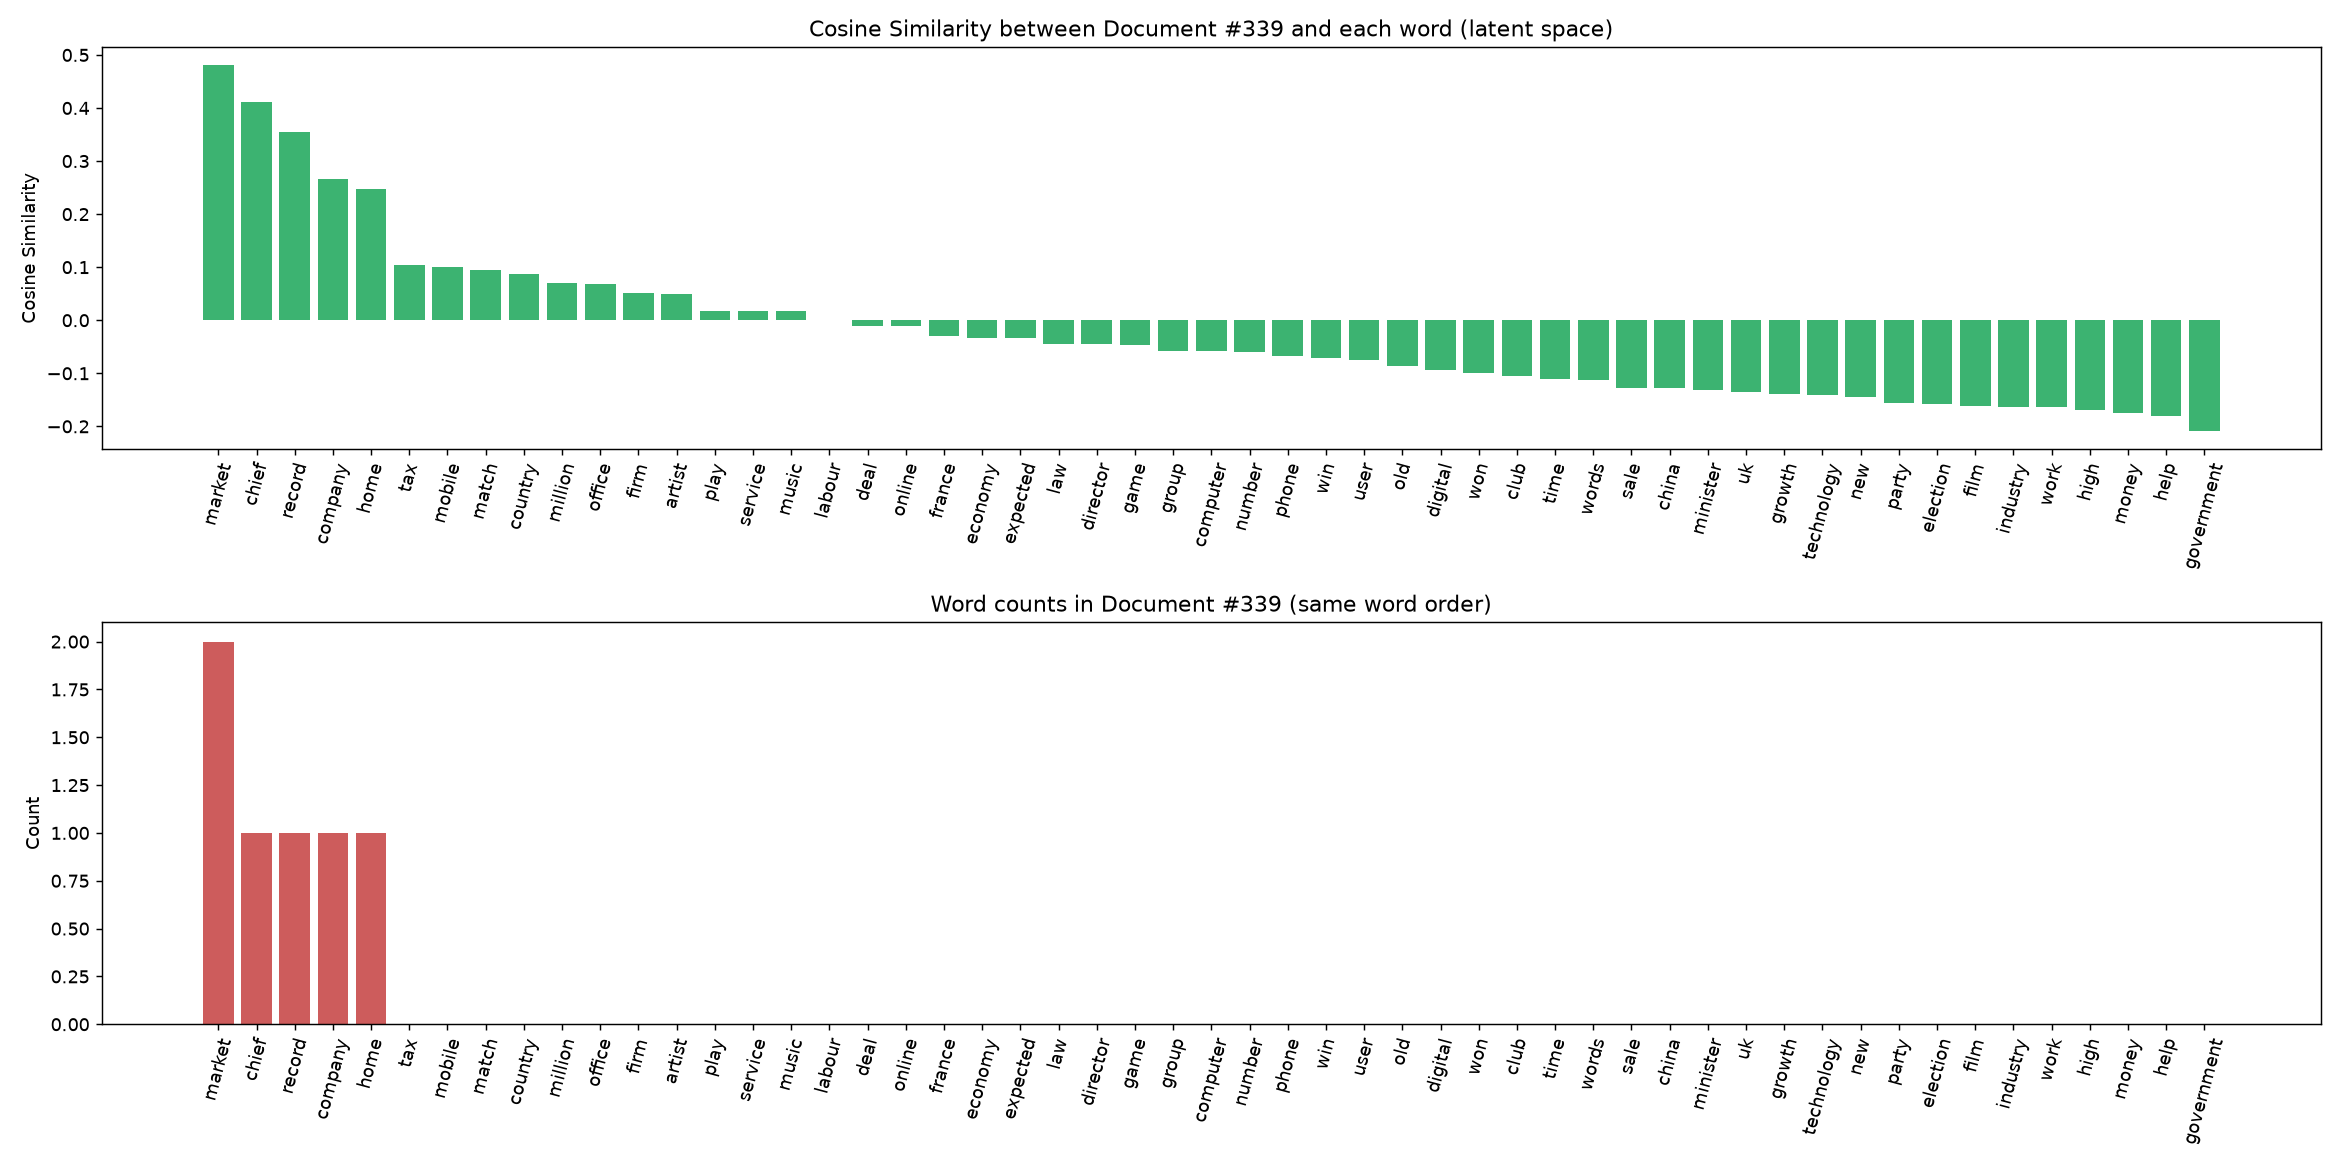
\includegraphics[width=1.0\textwidth]{q17_doc_similarity.png}
        \caption{نمودار بالایی: شباهت کسینوسی واژه‌ها با سند ۳۳۹ در فضای پنهان --- نمودار پایینی: تعداد تکرار واقعی همان واژه‌ها در سند}
        \label{fig:q17_doc_similarity}
    \end{figure}
\noindent
    تحلیل موازی این دو نمودار در شکل \ref{fig:q17_doc_similarity}، قدرت اصلی روش نمایه سازی معنایی نهان (\lr{Latent Semantic Indexing}) را آشکار می‌سازد:
    \begin{itemize}
        \item \textbf{انطباق فرکانسی کلمات کلیدی:}
        کلماتی مانند \lr{``market''} (۲ بار تکرار)، \lr{``chief''}، \lr{``record''}، \lr{``company''} و \lr{``home''} (هر کدام ۱ بار تکرار) در متن سند حضور داشته‌اند (نمودار قرمز). مدل SVD با موفقیت این کلمات را شناسایی کرده و بالاترین شباهت کسینوسی (بین $0.25$ تا $0.48$) را در فضای پنهان به آن‌ها اختصاص داده است (نمودار سبز).
        
        \item \textbf{کشف فراتر از کلمات موجود (تعمیم معنایی):}
        نکته بسیار حائز اهمیت این است که کلماتی مانند \lr{``tax''}، \lr{``mobile''}، \lr{``match''}، \lr{``country''} و \lr{``million''} با اینکه فرکانس حضور آن‌ها در نمودار پایینی **دقیقاً صفر** است، اما در نمودار بالایی شباهت کسینوسی مثبت و قابل توجهی (نزدیک به $0.1$) با سند دارند. 
        این پدیده به این دلیل است که سند شماره ۳۳۹ موضوعی مربوط به حوزه تجارت، شرکت‌ها و مسائل مالی داشته است. از این رو در فضای پنهان، بردارهای کلماتی مثل مالیات (\lr{tax}) یا ارزشی مانند میلیون (\lr{million}) به دلیل هم‌نشینی موضوعی همواره به بردار چنین سندی نزدیک می‌شوند؛ حتی اگر مستقیماً در متن آن سند نوشته نشده باشند.
        
        \item \textbf{جلوگیری از تداخل کلمات نامرتبط:}
        کلماتی مانند \lr{``government''}، \lr{``help''} و \lr{``money''} که شباهت کسینوسی منفی شدیدی با سند دارند، نشان‌دهنده‌ی مفاهیمی هستند که کاملاً متمایز از محور اصلی این سند بوده و مدل به درستی آن‌ها را پس زده است.
    \end{itemize}

\newpage

\noindent    \textbf{سوال ۱۹ --- تحلیل و تصویرسازی رفتار دسته‌ها در فضای پنهان با نقشه‌ی حرارتی (\lr{Heatmap})}
    
\noindent   در این گام، هدف این است که مشخص کنیم آیا فضای پنهان استخراج‌شده توسط SVD توانسته است مرزهای معنایی متمایزی بین دسته‌های مختلف خبری (مانند ورزش، سیاست، تجارت و...) ایجاد کند یا خیر. برای این کار، میانگین بردارهای اسناد متعلق به هر دسته محاسبه شده و به عنوان «امضای معنایی» آن دسته روی نقشه‌ی حرارتی ترسیم می‌شود. کد این بخش به صورت زیر است:

\begin{latin}
\begin{lstlisting}[language=Python]
# ============================================================
# Q19 — Mean Latent Space Vector per Category (Heatmap)
# ============================================================
def q19_category_heatmap(df_train, Uk, Sk, fname):
    doc_vecs = Uk * Sk
    
    categories = sorted(df_train['Label'].unique())

    mean_vecs = []
    for c in categories:
        mask = (df_train['Label'] == c).values
        mean_vecs.append(doc_vecs[mask].mean(axis=0))
        
    mean_vecs = np.array(mean_vecs)
    print(f"Mean latent vectors per category shape: {mean_vecs.shape}")

    fig, ax = plt.subplots(figsize=(14, 5))
    sns.heatmap(mean_vecs, cmap='coolwarm', center=0,
                yticklabels=[LABELS_MAP[c] for c in categories],
                xticklabels=[f'C{i+1}' for i in range(mean_vecs.shape[1])],
                ax=ax, cbar_kws={'label': 'Mean latent value'})
                
    ax.set_title('Mean Latent Space Vector per Category', fontsize=14)
    ax.set_xlabel('Latent Component', fontsize=12)
    
    plt.tight_layout()
    plt.savefig(f'media/{fname}.png', dpi=130)
    plt.close(fig)
    
    return mean_vecs
\end{lstlisting}
\end{latin}

    \subsection*{توضیح عملکرد متدها و منطق ریاضی:}

    \paragraph{۱. تشکیل ماتریس اسناد در فضای پنهان:}\hspace{-10pt}
    ابتدا با ضرب توزیعی سطر‌های ماتریس ویژگی‌های اسناد ($U_k$) در مقادیر منفرد متناظر آن‌ها ($\Sigma_k$)، نمایش واقعی اسناد در فضای کاهش‌یافته محاسبه می‌شود:
    $$D_{\text{latent}} = U_k \cdot \Sigma_k$$

    \paragraph{۲. محاسبه‌ی مرکز ثقل دسته‌ها (\lr{Centroid Calculation}):}\hspace{-10pt}
    برای هر دسته خبری $c$، یک ماسک منطقی روی داده‌ها اعمال می‌شود تا اسناد متعلق به آن طبقه تفکیک شوند. سپس میانگین هندسی این بردارها روی محور ستون‌ها (\lr{\texttt{axis=0}}) محاسبه می‌گردد تا یک بردار میانگین متمایز با ابعاد $1 \times 42$ به عنوان نماینده‌ی آن دسته حاصل شود:
    $$\vec{\mu}_c = \frac{1}{|D_c|} \sum_{d \in D_c} \vec{d}$$
    با تجمیع این بردارها برای تمام ۵ دسته، ماتریسی با ابعاد $5 \times 42$ تحت عنوان \lr{\texttt{mean\_vecs}} ساخته می‌شود.

    \paragraph{۳. رسم نقشه حرارتی با پالت رنگی دوقطبی:}\hspace{-10pt}
    نمودار با پالت رنگی \lr{\texttt{coolwarm}} ترسیم می‌شود که مرکز آن روی عدد $0$ تنظیم شده است. مقادیر مثبت (گرم/قرمز) نشان‌دهنده همبستگی مثبت شدید دسته با آن مؤلفه پنهان و مقادیر منفی (سرد/آبی) نشان‌دهنده تضاد یا همبستگی منفی است.

    \subsection*{تحلیل تجربی نقشه‌ی حرارتی و جدایی‌پذیری دسته‌ها:}\hspace{11pt}
    پس از اجرای الگوریتم، خروجی نمودار به شکل زیر در پوشه رسانه‌ها ذخیره می‌شود:

    \begin{figure}[h!]
        \centering
        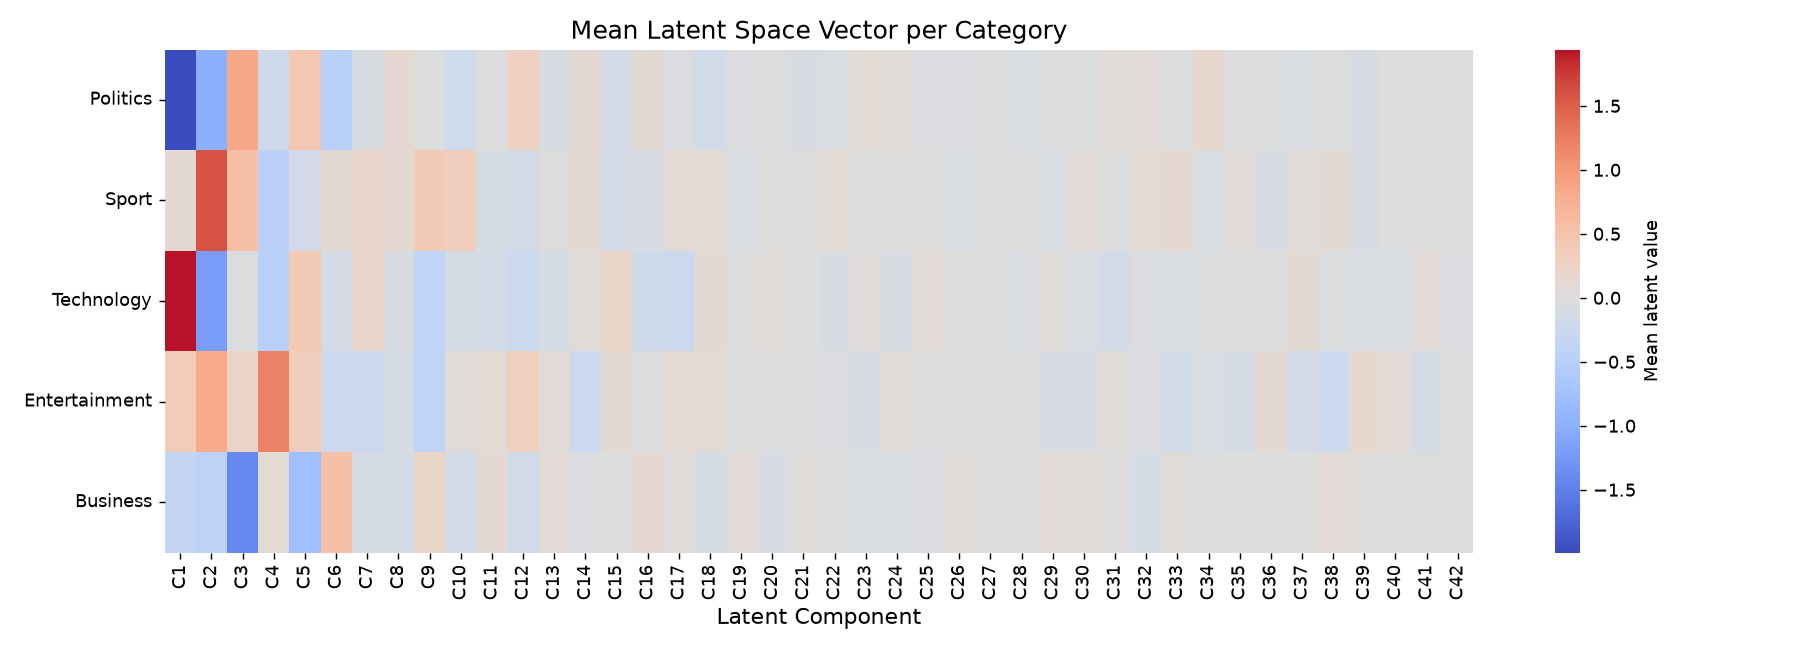
\includegraphics[width=1.0\textwidth]{q19_category_heatmap.png}
        \caption{نقشه‌ی حرارتی میانگین بردارهای پنهان به تفکیک ۵ دسته‌ی موضوعی اصلی}
        \label{fig:q19_category_heatmap}
    \end{figure}

    با تحلیل دقیق شکل \ref{fig:q19_category_heatmap}، نتایج شگفت‌انگیز زیر از توانایی جداسازی مفاهیم توسط LSI به دست می‌آید:
    \begin{itemize}
        \item \textbf{مرزبندی قوی دسته سیاست (\lr{Politics}) و فناوری (\lr{Technology}):} 
        مؤلفه اول پنهان ($C_1$) رفتار کاملاً متضادی را نشان می‌دهد؛ این مؤلفه برای موضوعات سیاسی به شدت منفی (آبی تیره) و برای موضوعات فناوری به شدت مثبت (قرمز تیره) است. این یعنی تنها با بررسی مقدار سند در مولفه‌ی اول ($C_1$) می‌توان با دقت بالایی اخبار سیاسی را از اخبار فناوری تفکیک کرد.
        
        \item \textbf{امضای اختصاصی ورزش (\lr{Sport}):}
        دسته ورزشی وابستگی شدیدی به مؤلفه دوم ($C_2$) دارد (رنگ قرمز تیره در سطر دوم). جالب اینجاست که در این مؤلفه، دسته‌های سیاست، فناوری و سرگرمی خنثی یا منفی هستند که نشان می‌دهد $C_2$ مشخصاً روی مفاهیم ورزشی متمرکز شده است.
        
        \item \textbf{تمایز حوزه سرگرمی (\lr{Entertainment}) و تجارت (\lr{Business}):}
        موضوعات هنری و سرگرمی بیشترین ثبت مقدار مثبت را روی مؤلفه چهارم ($C_4$) دارند، در حالی که موضوعات تجاری امضای اختصاصی خود را روی مؤلفه ششم ($C_6$) با رنگ نارنجی ملایم و همبستگی منفی شدید روی مؤلفه سوم ($C_3$) نشان می‌دهند.
        
        \item \textbf{پدیده میرایی مؤلفه‌های فرعی (کاهش واریانس):}
        اگر به ستون‌های سمت راست نمودار (از $C_{20}$ تا $C_{42}$) نگاه کنیم، رنگ غالب به سمت خاکستری بی‌اثر (نزدیک به صفر) متمایل می‌شود. این رفتار کاملاً با تئوری SVD همخوانی دارد؛ چرا که مقادیر منفرد به صورت نزولی مرتب شده‌اند و مؤلفه‌های انتهایی واریانس و اطلاعات بسیار کمتری از توزیع داده‌ها را حمل می‌کنند.
    \end{itemize}

\noindent\textbf{سوال ۲۰ --- ارزیابی تجربی مدل دسته‌بندی نزدیک‌ترین مرکز ثقل (\lr{Nearest Centroid Classifier}) در فضای پنهان}
    
\noindent    در گام پایانی پروژه، یک مدل دسته‌بندی معنایی بر پایه محاسبات هندسی طراحی شده است. این مدل، هر سند جدید از مجموعه‌ی تست (\lr{Test Set}) را به فضای پنهان منتقل کرده و با سنجش شباهت کسینوسی آن با مرکز ثقل (\lr{Centroid}) هر یک از دسته‌های پنج‌گانه در داده‌های آموزش، دسته‌ی پیش‌بینی‌شده را تعیین می‌کند. کد این بخش به صورت زیر است:

\begin{latin}
\begin{lstlisting}[language=Python]
# ============================================================
# Q20 — Multi-class Classification & Evaluation
# ============================================================
def cosine_sim_matrix(A, B):
    A_norm = A / np.linalg.norm(A, axis=1, keepdims=True)
    B_norm = B / np.linalg.norm(B, axis=1, keepdims=True)
    return A_norm @ B_norm.T

def q20_evaluate(df_train, bow_train, df_test, bow_test, scaler, Vtk):
    X_train_scaled = scaler.transform(bow_train.astype(float))
    doc_latent_train = X_train_scaled @ Vtk.T

    categories = sorted(df_train['Label'].unique())
    centroids = np.array([
        doc_latent_train[(df_train['Label'] == c).values].mean(axis=0)
        for c in categories
    ])

    X_test_scaled = scaler.transform(bow_test.astype(float))
    doc_latent_test = X_test_scaled @ Vtk.T

    sims = cosine_sim_matrix(doc_latent_test, centroids)
    preds = np.array(categories)[np.argmax(sims, axis=1)]
    true = df_test['Label'].values

    acc_overall = (preds == true).mean()
    print(f"Overall accuracy: {acc_overall:.4f}  (n={len(true)})")
    for c in categories:
        mask = true == c
        if mask.sum() > 0:
            acc_c = (preds[mask] == true[mask]).mean()
            print(f"  {LABELS_MAP[c]:<15} n={mask.sum():<5} acc={acc_c:.4f}")
        else:
            print(f"  {LABELS_MAP[c]:<15} n=0 (not present in this test split)")
    return acc_overall
\end{lstlisting}
\end{latin}

    \subsection*{توضیح عملکرد متدها و منطق محاسباتی مدل:}

    \paragraph{۱. ضرب ماتریسی بهینه‌ی تشابه کسینوسی (\lr{\texttt{cosine\_sim\_matrix}}):}\hspace{-10pt}
    برای جلوگیری از به‌کارگیری حلقه‌های تکرار کند پایتون، ابتدا سطرهای ماتریس‌های $A$ و $B$ با تقسیم بر نرم اقلیدسی‌شان پیش‌نرمال‌سازی می‌شوند. ضرب ماتریسی حاصل‌ضرب این دو ماتریس نرمال‌شده (\lr{\texttt{A\_norm @ B\_norm.T}})، به طور هم‌زمان تشابه کسینوسی تمام اسناد تست را با تمام مراکز ثقل محاسبه می‌کند.

    \paragraph{۲. انتقال داده‌های تست به فضای کاهش‌یافته:}\hspace{-10pt}
    با مجهز بودن به ماتریس راست مفرد $V_k^T$ که از داده‌های آموزش استخراج شده است، ابتدا فرکانس اسناد تست با میانگین و انحراف معیار داده‌های آموزش استانداردسازی (\lr{\texttt{scaler.transform}}) شده و سپس با نگاشت خطی زیر به فضای ۴۲ بعدی منتقل می‌شوند:
    $$D_{\text{test\_latent}} = X_{\text{test\_scaled}} \cdot V_k^T$$

    \paragraph{۳. قانون تصمیم‌گیری مرکز ثقل:}\hspace{-10pt}
    هر سند تست به دسته‌ای تخصیص می‌یابد که بیشترین شباهت کسینوسی (زاویه نزدیک‌تر به مرکز ثقل در زیرفضای پنهان) را با آن داشته باشد:
    $$\hat{y} = \arg\max_{c \in \{1, \dots, 5\}} \text{CosineSimilarity}(\vec{d}_{\text{test}}, \vec{\mu}_c)$$

    \subsection*{تحلیل تجربی نتایج دسته‌بندی روی مجموعه داده تست:}
    پس از اجرای نهایی ارزیابی روی ۲۲۵ سند تست، نتایج زیر حاصل شده است:

    \begin{figure}[h!]
        \centering
        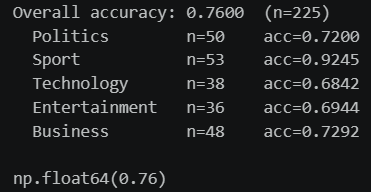
\includegraphics[width=0.6\textwidth]{Output20.png}
        \caption{دقت کلی و تفکیک‌شده‌ی مدل دسته‌بندی نزدیک‌ترین مرکز ثقل در فضای پنهان SVD}
        \label{fig:q20_evaluation_output}
    \end{figure}

    با تحلیل خروجی ثبت‌شده در شکل \ref{fig:q20_evaluation_output}، کارآمدی هندسی مدل را بررسی می‌کنیم:
    \begin{itemize}
        \item \textbf{دقت کلی قابل قبول (\lr{Overall Accuracy}):}
        مدل دسته‌بندی بسیار ساده و بدون پارامتر ما موفق شده است به دقت کل \textbf{\%۷۶.۰۰} روی کل داده‌های تست ($n=225$) دست یابد. این موضوع نشان می‌دهد تقلیل ابعاد به کمک SVD، واریانس‌های مزاحم و نویزهای متنی را حذف کرده و ساختار متمایز هندسی کلمات و اسناد را به خوبی حفظ کرده است.

        \item \textbf{عملکرد درخشان در حوزه ورزش (\lr{Sport}):}
        دسته ورزشی با داشتن ۵۳ سند تست به دقت بی‌نظیر \textbf{\%۹۲.۴۵} رسیده است. با تطابق این یافته با نتایج سوال قبل (نقشه حرارتی)، متوجه می‌شویم اسناد ورزشی رفتار به شدت متمرکزی روی مؤلفه دوم ($C_2$) دارند و مرکز ثقل آن‌ها به شدت در فضای پنهان منزوی و متمایز از سایر دسته‌هاست که طبقه‌بندی آن را تسهیل می‌کند.

        \item \textbf{چالش‌های دسته‌بندی در سایر حوزه‌ها:}
        کمترین میزان دقت مربوط به دسته‌‌ی فناوری (\lr{Technology}) با مقدار \textbf{\%۶۸.۴۲} و سرگرمی (\lr{Entertainment}) با مقدار \textbf{\%۶۹.۴۴} است. این افت نسبی به علت هم‌پوشانی لغوی برخی مستندات تفریحی و بازی‌های آنلاین با تکنولوژی دیجیتال است که در ابعاد پنهان مرزهای نزدیک‌تری به یکدیگر دارند. با این حال، دستیابی به دقت نزدیک به \%۷۰ با استفاده از یک مدل پایه مبتنی بر مرکز ثقل، نشان‌دهنده‌ی کارایی بالای ریاضیات جبر خطی در مدیریت معنایی داده‌های متنی است.
    \end{itemize}

\end{document}